\documentclass[usenatbib,fleqn]{mnras}

\makeatletter
\newlength{\abovecaptionskip}%
\setlength{\abovecaptionskip}{10\p@}
\makeatother


\usepackage{threeparttable}
 

\usepackage{amsmath,amssymb}
\usepackage{mathrsfs}
\usepackage{graphicx}
\usepackage{epstopdf}
%\usepackage{hyperref}
\epstopdfsetup{outdir=./figures/}
\graphicspath{{./figures/}}
\usepackage{url}
%\usepackage{aas_macros}

\newcommand\lsim{\mathrel{\rlap{\lower4pt\hbox{\hskip1pt$\sim$}}
    \raise1pt\hbox{$<$}}}
\newcommand\gsim{\mathrel{\rlap{\lower4pt\hbox{\hskip1pt$\sim$}}
    \raise1pt\hbox{$>$}}}


\newcommand       \be          {\begin{eqnarray}}
\newcommand       \ee          {\end{eqnarray}}
\newcommand{\Mbh}[1][]{M_{\bullet#1}}
\newcommand{\Menc}{M_{\rm enc}}
\renewcommand{\th}{t_h}
\newcommand{\Msun}{{\rm M_\odot}}
\newcommand{\pyear}{{\rm yr}^{-1}}

% write title (with email and institute)
\title{Are tidal disruption event jets hiding?}
\author[Generozov et al.]{ A. Generozov$^{1}$, P. Mimica$^{2}$,
  B. D. Metzger$^{1}$,
  D. Giannios$^{3}$, 
  N. Stone$^{1}$,
  M.A. Aloy$^{2}$ 
  \\
  $^{1}$Columbia Astrophysics Laboratory, Columbia University, 550 West 120th Street, New York, NY 10027\\
  $^{2}$Departamento de Astronomia y Astrofisica, Universidad de Valencia, E-46100 Burjassot, Spain\\
  $^{3}$Department of Physics and Astronomy, Purdue University, 525
  Northwestern Avenue, West Lafayette, IN 47907, USA}

\begin{document}
\maketitle
\begin{abstract}
  There are now dozens of candidates for tidal disruptions of stars by
  supermassive black holes (TDEs) in optical and x-rays. A small
  fraction of these events, (e.g. Sw-J1644+57) have radio emission
  consistent with a powerful, relativistic jet interacting with
  surrounding nuclear gas. A priori it is not clear if the small
  number of observed relativistic TDEs is due to an intrinsic lack of jets
  or unfavorable nuclear gas densities for producing observable radio
  emission. We test the second possibility by calculating radio
  light-curves for jets interacting with a broad range of density
  profiles, bracketing the expected range of gas densities in galactic
  nuclei (1-1000 cm$^{-3}$ at $10^{18}$ cm). We find bright radio
  transients across the entire range of expected density
  profiles. Existing radio upper limits are often taken decades after
  the observed flare, well after the expected peak of the light-curve
  for low density environments. Nonetheless they exclude powerful,
  Sw-J1644-like jets for CNM densities less than 60 cm$^{-3}$ at
  $10^{18}$ cm. More stringent constraints would be possible with
  prompt follow-up of tidal disruption event candidates and would
  inform our understanding jet launching physics.
\end{abstract}
\section{Introduction}
\label{sec:intro}
When a star in a galactic nucleus is deflected too close to the
central supermassive black hole (BH), it can be torn apart by tidal
forces.  During this tidal disruption event (TDE), roughly half of the
stellar debris remains bound to the BH, while the other half is flung
outwards and unbound from the system.  The bound material, following a
potentially complex process of debris circularization
(\citealt{Guillochon+2013},\citealt{Hayasaki+2013},\citealt{Hayasaki+2015},\citealt{Shiokawa+2015},\citealt{Bonnerot+2015}),
accretes onto the BH, creating a luminous flare lasting months to
years \citep{Hills1975, Carter+1982, Rees1988}.

Many thermal TDE flares have now been identified at UV/optical
\citep{van-Velzen+2011, Gezari+2012, Chornock+2014, Arcavi+2014} and
soft x-ray wavelengths \citep{Esquej+2007}.  Beginning with the
discovery of {\it Swift} J1644+57 in 2011, three additional TDEs have
been discovered by their non-thermal x-ray emission
(\citealt{Bloom+2011, Levan+2011, Burrows+2011, Zauderer+2011,
  Cenko+2012, Pasham+2015, Brown+2015}).  Unlike the thermal TDEs,
these events are the result of emission from a transient relativistic
jet beamed along our line of sight, similar to the blazar geometry of
active galactic nuclei (AGN).  In addition to their highly variable
X-ray emission, which likely originates from the base of the jet,
these events are characterized by radio synchrotron emission.  The
latter, more slowly evolving, is powered by shocks formed at the
interface between the jet and surrounding circumnuclear medium (CNM)
(\citealt{Giannios&Metzger2011,Metzger+2012}), analagous to the
afterglow of a gamma-ray burst.

Although a handful of jetted TDE flares have been observed, their
volumetric rate is a very small fraction $\sim 10^{-4}$ of the rate of
the observed thermal TDE flares (e.g., \citealt{Burrows+2011}), and an
even smaller fraction of the theoretically predicted TDE rate
(\citealt{Stone&Metzger2016}).  One potential explanation for this
discrepancy is that the majority of TDEs produce powerful jets, but
their non-thermal X-ray emission is relativistically beamed into a
small angle $\theta_{\rm b}$, making them visible to only a small
fraction of observers.  However, in order to explain the required
beaming fraction $f_b \approx \theta_{b}^{2}/2 \sim 10^{-4}$ would
require $\theta_{\rm b} \sim 0.01$ and hence a jet with a bulk Lorentz
factor of $\Gamma \gtrsim 1/\theta_j \sim 100$, much higher than
typically inferred for AGN jets or inferred for {\it Swift} J1644+57
(\citealt{Metzger+2012}).

The low detection rate of non-thermal TDE may instead indicate that
jets are intrinsically rare in TDEs, or the conditions of the
surrounding environment are unfavorable for producing bright emission.
Jets could be rare if they require, for instance, a highly
super-Eddington accretion rate (\citealt{De-Colle+2012}), a TDE from a
deeply plunging stellar orbit (\citealt{Metzger&Stone2015}), or a
particularly strong magnetic flux threading the star
(\citealt{Tchekhovskoy+2014,Kelley+2014}).  Alternatively, jet formation
or its X-ray emission could be suppressed if the disk undergoes
Lens-Thirring precession due to a misalignment between the angular
momentum of the BH and that of the disrupted star
(\citealt{Stone&Loeb2012}).  In the latter case, however, even a `messy'
jet could still be produced, which emits luminous non-thermal radio
synchrotron emission as it interacts the surrounding CNM.  The radio
emission from an off-axis is predicted to be relatively isotropic
(\citealt{Giannios&Metzger2011},\citealt{Mimica+2015}).

Observational campaigns have been conducted to follow-up thermal TDE
flares at radio wavelengths on timescales of months to decades after
the outburst (\citealt{Bower+2013}; \citealt{van-Velzen+2013}; see Table
1 of \citet{Mimica+2015} for a compilation).  \citet{van-Velzen+2013}
detected no radio emission from their 7 candidates, while
\citet{Bower+2013} detected radio emission from two of the  ROSAT flares:
RX J1420.4+5334 and IC 3599.  However, for RX J1420.4+5334 the radio
emission was observed in a different galaxy than that originally
identified by \citet{Komossa+1999} as the host.  Furthermore, the
highly irregular behavior of IC 3599, including multiple outbursts
over the past few decades from this low luminosity AGN
(e.g.~\citealt{Campana+2015}), calls into question whether this event is
a true TDE at all.  \citet{Bower+2013} and \citet{van-Velzen+2013} use a
simple model for the radio emission as a Sedov blast wave, to conclude
that $\lesssim 10\%$ of TDEs produce jetted TDE emission at a level
similar to that produced in {\it Swift} J1644+57.  \citet{Mimica+2015}
used 2D hydrodynamical models, coupled with a synchrotron radiation
transport calculation, to model the on-axis emission from {\it Swift}
J1644+57, which they then extended to the case of an off-axis viewing
angle to conclude that most previous TDEs should have been detected if
their jets were as powerful.

Previous works (\citet{Bower+2013}; \citet{van-Velzen+2013};
\citealt{Mimica+2015}) have generally assumed that all TDEs occur in a
similar environment as {\it Swift} J1644+57.  However, in general the
gas density in a galactic nucleus depends sensitively on the sources
of gas from stellar winds, and the sources of gas heating
(\citealt{Quataert2004},\citealt{Generozov+2015}).  In a gamma-ray
burst, the environment the jet emerges is relatively well-understood
to be the wind of the massive progenitor star, or the ISM of the host
galaxy.  However, in a TDE, the density could in principle be orders
of magnitude higher.

In this paper we address the range of gas densities encountered by
jetted TDEs and estimate their synchrotron emission by means of
analytic calculations and numerical simulations.  If we find radio
emission should be detected for all plausible CNM densities, then we
are lead to the conclusion that most TDEs do not launch J1644-like
jets.  This result would have significant implications for the physics
of jet launching in TDEs and more broadly.

In $\S\ref{sec:cnm}$ we explore the expected CNM densities using the
formalism developed in \citet{Generozov+2015} (hereafter GSM15) to
calculate the CNM profile for different assumptions about the stellar
population in the galactic nucleus.  A younger stellar population
produces significant wind mass loss from O \& B stars. In contrast,
the rate of wind mass loss from an older population, which lacks these
massive stars, could $\sim 2$ orders of magnitude smaller.  We show
that the requirement of a physical stellar population, combined with
condition of thermal stability of the hot gas phase, limits the gas
density on a scale of $10^{18}$ cm to a range of $n_{18} \sim
1-10^{3}$ cm$^{-3}$.  Although these limits come from considering
only the hot phase of gas, we show based on the measured distribution
of Eddington ratios that the average density in most galactic nuclei
is bracketed by this range. 

As a second component of this paper, in $\S\ref{sec:jet}$ we
explore the expected synchrotron emission from J1644+57-like across
the allowed range of CNM conditions.  We start in
$\S\ref{sec:analytic}$ with analytic conditions.  Then in
$\S\ref{sec:numerical}$ use both 1d and 2d hydrodynamic models to
simulate the jet propagating through the CNM and compare the results
in $\S\ref{sec:2d}$. In $\S\ref{sec:results}$ we show radio
light-curves from our 1d models for a wide range of CNM densities, to
illustrate qualitatively how much varying the CNM density by itself
could change the radio light-curve.  We summarize our conclusions in
$\S\ref{sec:conc}$.

\section{Range of CNM Densities}
\label{sec:cnm}

In this section we place theoretical and observational constraints on
the radial profile of the gas density $n(r)$ in the nuclei of
galaxies, which typically takes on a power-law form $n =
n_{18}(r/10^{18}{\rm cm})^{-\gamma}$ with $\gamma \approx 1-1.5$.  We
focus constraining the normalization $n_{18}$ of the density at $r =
10^{18}$ cm, as the latter represents the approximate deceleration
radius of the blast wave ($\S\ref{sec:analytic}$)

\subsection{Analytic Constraints on CNM Density}

\subsubsection{CNM Model}
\label{sec:model}

The dominant source of gas injection into the CNM of quiescent
galaxies is winds from stars in the galactic nucleus. The 1D spherical
hydrodynamic equations with stellar wind mass injection are
(e.g. \citealt{Holzer+1970}; \citealt{Quataert2004}) 
\begin{align}
  &\frac{\partial \rho}{\partial t}+\frac{1}{r^2}\frac{\partial}{\partial r}\left(\rho r^2 v\right)=q \label{eq:drhodt}\\
  &\rho \left(\frac{\partial v}{\partial t} + v\frac{\partial
      v}{\partial r}\right) =-\frac{\partial p}{\partial r}- \rho\frac{GM_{\rm enc}}{r^{2}} -q v \label{eq:dvdt}\\
  &\rho T\left(\frac{\partial s}{\partial t} + v\frac{\partial
      s}{\partial
      r}\right)=q\left[\frac{v^2}{2}+\frac{v_w^2}{2}-\frac{\gamma}{\gamma-1}
    \frac{p}{\rho} \right] ,
\label{eq:dsdt}
\end{align}
where $\rho = \mu m_p n$, $v$, $p$, and $s$ are the density, velocity,
pressure (assumed to be an ideal gas with $\mu = 0.62$), and specific
entropy, respectively.  The enclosed mass $\Menc = M_{\bullet} +
M_{\star}$ includes both the black hole mass $M_{\bullet}$ and
enclosed stellar mass $M_{\star} \propto \int \rho_{\star}r^{2}dr$.

The mass source term $q =\eta \rho_\star/\th$ is the mass injection
rate per unit volume per unit time, where $\rho_\star$ is the stellar
density.  At small radii of interest, inside the Nuker `break' radius,
the stellar density follows $\rho_\star\sim r^{-\delta_1}$, where
$\delta_1 = 1-2$ is the inner Nuker profile \citep{Lauer+2007}.  The
energy source term $\propto v_w^{2}$ parameterizes the heating rate of
the gas, as physically results from stellar wind kinetic energy,
supernovae, and black hole feedback.

For a cusp galaxy ($\delta_1> 0.5$), \citet{Generozov+2015} show that the gas density obeys $n \sim
r^{-1}$, with a normalization
\begin{equation}
n_{18}\simeq 0.4 \Mbh[,7]^{0.5} \eta_{0.02} v_{500}^{-1.5} {\rm
  cm^{-3}},
\label{eq:n18}
\end{equation}
where $\Mbh[,7]= \Mbh/10^7 \Msun$,
$\eta_{0.02}= \eta/0.02$, and $v_{500}=v_w/500$ km s$^{-1}$, and we have assumed a fixed slope for the stellar density
power law slope $\delta_1=1.8$. 

Equation (\ref{eq:n18}) shows that the gas density is sensitive to the
mass return parameter and the heating rate, which are related to the
star formation history. Young, massive stars put out very energetic
winds with $v_w\simeq 1000$ km s$^{-1}$ with a high mass return rate,
$\eta\simeq 100$.  In contrast, stars with age comparable to that of
the universe will have slow winds with speeds of order\footnote{In the
  case of such low heating, $v_w \lesssim \sigma$, the heating of the
  gas is dominated by the velocity dispersion of the nucleus
  $\sigma$.} $\sim 10$ km s$^{-1}$ and mass return parameters,
$\eta\simeq0.02$. We will explore the range of mass
return parameters, heating rates, and gas densities allowed by
plausible star formation histories in $\S$~\ref{sec:densAllowed}.

\subsubsection{Gas density profiles}
The slope of the gas density profile depends on the slope of the
stellar density profile.  This is because the  mass source function is
proportional to the stellar density (see~\ref{sec:model}). There are
two broad categories of stellar density profiles: ``cusps'', with power
law slopes $>$ 0.5  and ``cores'', with power law slopes $<0.3$ \citep{Lauer+2007}.

We show example steady state gas density profiles for a cusp and a
core stellar density profiles in Fig.~\ref{fig:profiles}. The cusp
(core) profile has $\rho_\star \propto r^{-1.8 (-1.1)}$ for $r < 25$
pc. Both have $\rho_\star \propto r^{-3}$ for $r > 25$ pc.

For the cusp profile the gas density $\rho \propto r^{-1}-r^{-1.1}$
inside of break in stellar density (25 pc).  The core profile
is similar to the cusp galaxy for $r<10^{18}$ cm. However, it flattens near
$10^{18}$ cm.  The radius where the core profile flattens corresponds
to the stagnation radius, $r_s$, where the gas velocity goes through
0.  $r_s$ depends on the model parameter ($\Mbh$ and $v_w$--see
GSM15).

Both gas density profiles steepen at the stellar break
radius. In general, there will be breaks in the gas density slope
wherever there are breaks in the stellar density slope (since the mass
source function is proportional to the stellar density).  Integrated
light profiles of galactic nuclei are well fit by broken power laws,
but the characteristic break radius is typically larger than $5 $ pc
\citep{Lauer+2007}. However, if a nuclear star cluster is present
there would be a small effective break at the outer edge of the
cluster, typically 1-5 pc \citep{Georgiev+2014}.

We expect breaks in the gas density profile will only be important
inside of the Sedov radius, where it has swept up its own mass in CNM
gas.  The jet mostly decelerates inside of this radius, becoming
Newtonian and so the profile outside of this radius will be of minimal
importance in shaping the radio light-curve. We plot the Sedov
radius for different energy jets on each of the profiles in
Fig.~\ref{fig:profiles}. For realistic break radii $\gsim 1$ pc and
our fiducial $E_{54}=4$, the break radius will only be important for
small densities ($n_{18}<20$). Henceforward we will not consider the
effects of the break radius in our analysis.

From Fig.~\ref{fig:profiles}, the gas density profile for a cusp
galaxy is approximately

\begin{equation}
n(r) \approx n_{18} \left(\frac{r}{10^{18} {\rm cm}}\right)^{-1}
\label{eq:cuspProfile}
\end{equation}

inside of the break radii. As we expect, cusp galaxies to dominate the
tidal disruption event rate \citep{Stone&Metzger2016}, we adopt
equation~\eqref{eq:cuspProfile} as our fiducial CNM density profile.

We also experiment with a core-like density profile
(appendix~\ref{app:core}), and compare the radio light-curves for jets
going through core and cusp-like density profiles in
$\S\ref{sec:profileComp}$.


\begin{figure}
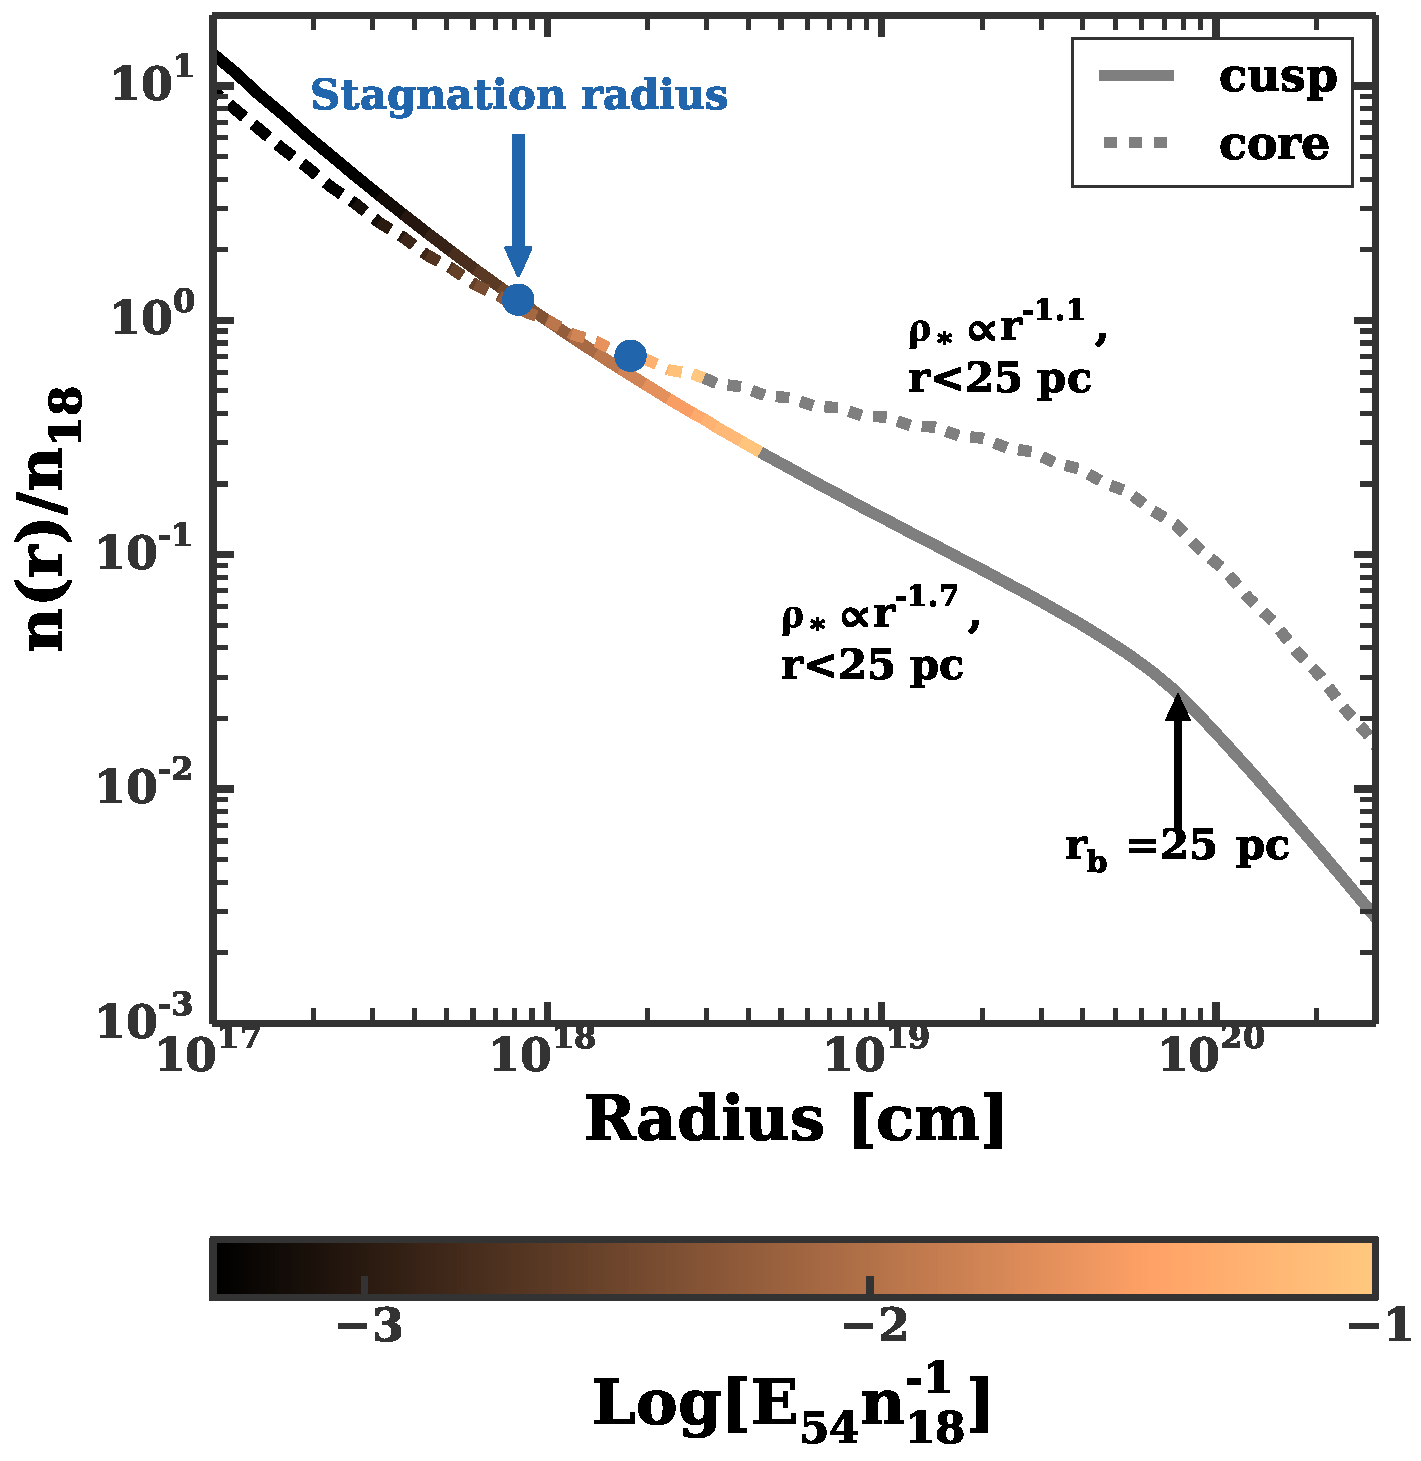
\includegraphics[width=8cm]{sedov_radius.pdf}
\caption{\label{fig:profiles} Steady state core and cusp density
  profiles. We have taken $\Mbh=10^{7} \Msun$ and $v_w$=600 km/s and
  both profiles have mass source function $q(r) \propto
  r^{-3}$ for $r > 25$. The core profile has $q(r) \propto
  r^{-1.1}$ for $r < 25$ and the cusp profile has $q(r)
  \propto r^{-1.8}$.  The colors at each radius indicate the value of
  isotropic jet energy $E_{52} n_{18}^{1}$, such that the gas mass
  inside that radius is equal to the mass inside the jet. We take the
  Lorentz factor of the un-shocked jet to be $\gamma_{\rm jet}=2$.}
\end{figure}



\subsubsection{Allowed Density Range}
\label{sec:densAllowed}

Equation (\ref{eq:n18}) shows that increasing the mass return
parameter, $\eta$, or decreasing the heating parameter $v_w$,
increases the gas density, $n_{18}$.  However, as we now show, one
cannot increase the $\eta$ or decrease $v_w$ indefinitely, as the CNM
will become thermally unstable.  Defining thermally instability as
occuring when the cooling time of the gas is less than 10 times the
local dynamical timescale (\citealt{McCourt+2012}), GSM15 show that the
CNM is thermally unstable for wind heating rates below a critical
value
\begin{equation}
v_{\rm w,TI}\simeq 200 \eta_{0.02}^{0.17} \Mbh[,7]^{0.08} \,{\rm km \,\,s^{-1}},
\label{eq:ti}
\end{equation}
where we have assumed line cooling dominates free-free emission, as is valid for $v_{\rm w} \lesssim 10^{3}$ km s$^{-1}$.

If the hot phase of CNM reaches a thermally unstable condition
($v_{\rm w} \lesssim v_{\rm w,TI}$), it is likely that portions of the
hot phase will condense into cold gas, eventually resulting in star
formation.  Therefore, it is reasonable to hypothesize that the CNM
will regulate itself to the condition $v_w \gsim v_{\rm w,TI}$ (a
similar argument has been made on larger scales in galaxies;
\citealt{Voit+2015}).  The condition places an upper limit on the gas
density
\begin{equation}
n_{18} \lesssim n_{\rm 18,TI}\simeq 1.6 \eta_{0.02}^{0.75} \Mbh[,7]^{0.38} \, {\rm cm^{-3}}\,\,\,\text{Thermal Stability}
\label{eq:n18ti},
\end{equation}
where we have used equations~\eqref{eq:n18} and~\eqref{eq:ti}.

The maximum physical value of $\eta\simeq 400$ occurs $\sim 3$ Myr after a burst of star formation.\footnote{For details
  of how to calculate $\eta$ for a given star formation history see
  appendix C of \citet{Generozov+2015}.}  Evaluating equation~\eqref{eq:n18ti} with
$\eta=400$ gives the maximum thermally-stable CNM density
\begin{equation}
n_{\rm 18,max} \simeq 2.7\times 10^{3} \Mbh[,7]^{0.38} {\rm cm^{-3}}
\label{eq:n18max}
\end{equation}

Although such a large gas density would be present in the immediate
aftermath of a starburst, the wind mass loss rate (and hence the gas
density) declines as $\eta \sim t^{-3}$. Thus we expect the gas
density would decline by an order of magnitude after just a few Myr. Note
that type II Supernovae could inject additional mass into the CNM, but
this injection would be intermittent (e.g. the time between SNe is
long compared to a dynamical time for the scales of interest).

What is the smallest plausible CNM density? This would correspond to a
small mass return parameter and a high heating rate. The mass return
parameter, $\eta=0.02$, reaches its minimum value for a stellar
population that is a Hubble time old. A stellar population
that is $<$ 3 Myr old will have a heating rate, $v_w=3,000$ km s$^{-1}$.

A stellar population in which a small fraction, $f$ of the stars
formed $\lsim 3$ Myr ago and the rest are a Hubble time old, will have
both a high heating rate and a low mass return rate. In this scenario
$n_{18}$ will be minimized for $f=4\times 10^{-4}$. Both old and young
stars contribute significantly to the mass injection rate giving
$\eta\simeq 0.03$, while the young star dominate the heating
$v_w\simeq 3,000$ km/s and thermally stabilize the gas. These
parameters provide the minimum possible CNM gas density
\begin{equation}
n_{\rm 18,min}\simeq 0.06 \Mbh[,7]^{0.5} {\rm cm^{-3}}
\label{eq:n18min}
\end{equation}

We illustrate how the mass return parameter, heating rate, and density
vary with star formation history in Fig.~\ref{fig:param}. The solid
gray line represents a two-burst model for star formation in which a
fraction, $f$, of the stars formed $<$ 3 Myr ago and the remainder
formed a Hubble time ago.  Towards the top right the
$f=1$ and the young stars dominate the mass injection rate and the
heating rate.  Moving towards the left, $f$ decreases, along with the
mass return rate, and density (blue lines), but the heating rate,
$v_w$, remains $\gsim 1000$ km/s except for very small values of
$f$. The minimum density (eq.~\eqref {eq:n18min}) is obtained for
$f=4\times 10^{-4}$. However, for this $f$, we expect less than 1
massive star within the stagnation radius. In this case our formalism
would break down, and the true density would be larger. For a simple
estimate we set the location of the stagnation radius by requiring it
enclose ten massive stars, we obtain a density of $n_{18} \sim$ 3
cm$^{-3}$ (note we assume $n\sim r^{-1}$). Thus, the minimum plausible
$n_{18}$ is $\sim$ few cm$^{-3}$.  

The dashed, gray line represents another two burst formation history
but the older burst is $\sim 3$ Myr old (when stars are beginning to
leave the main sequence), increasing the mass injection rate. Towards
the lower right of the dashed, gray line these somewhat older stars
dominate the mass injection into the CNM, increasing the density
towards the the thermal instability threshold (thick, black line). The
intersection between the dashed gray line and the thermal instability
line corresponds to the maximum possible hot phase CNM density.

A typical host galaxy for TDE has evidence of some star formation
within 1 Gyr \citep{French+2016}. In this case
the return efficiency will be $\eta\simeq 0.4$. The heating is
dominated by the stellar velocity dispersion Ia supernovae.  Gas will
be inflowing inside of the Ia radius, where the time between
supernovae is equal to the dynamical time: for $10^7 \Msun$ and this
will be $\simeq 10$ pc. Then,

\begin{equation}
n_{\rm Ia}=\frac{t_{\rm dyn}(r_{\rm Ia}) \left[\eta M_{\star} (r_{\rm
    Ia})/t_h\right]}{4 \pi/3 r_{\rm Ia}^3 m_p}
\label{eq:nIa}
\end{equation}

$t_{\rm dyn}(r_{\rm Ia})=(G \Mbh/r_{\rm Ia}^3)^{-1/2}$ is the
dynamical time at Ia radius. $M_{\star}(r_{\rm Ia})$ is the stellar
mass enclosed inside the Ia radius:

\begin{align}
&\Mbh (r_{\rm Ia}/r_{\rm inf})^{3-\delta}\\
&r_{\inf}\approx 3.5 \Mbh[,7]^{0.6} \, {\rm pc}
\end{align}

$r_{\rm inf}$ is the influence radius and $\delta$
is power law slope of the stellar density profile. Overall, we obtain
a density of $n_{\rm Ia} \simeq 1 \, {\rm cm}^{-3}$ at the Ia
radius. Assuming $n\propto r^{-1}$ we obtain $n_{18}\simeq 50$ cm$^{-3}$. 

 

\begin{figure} 
  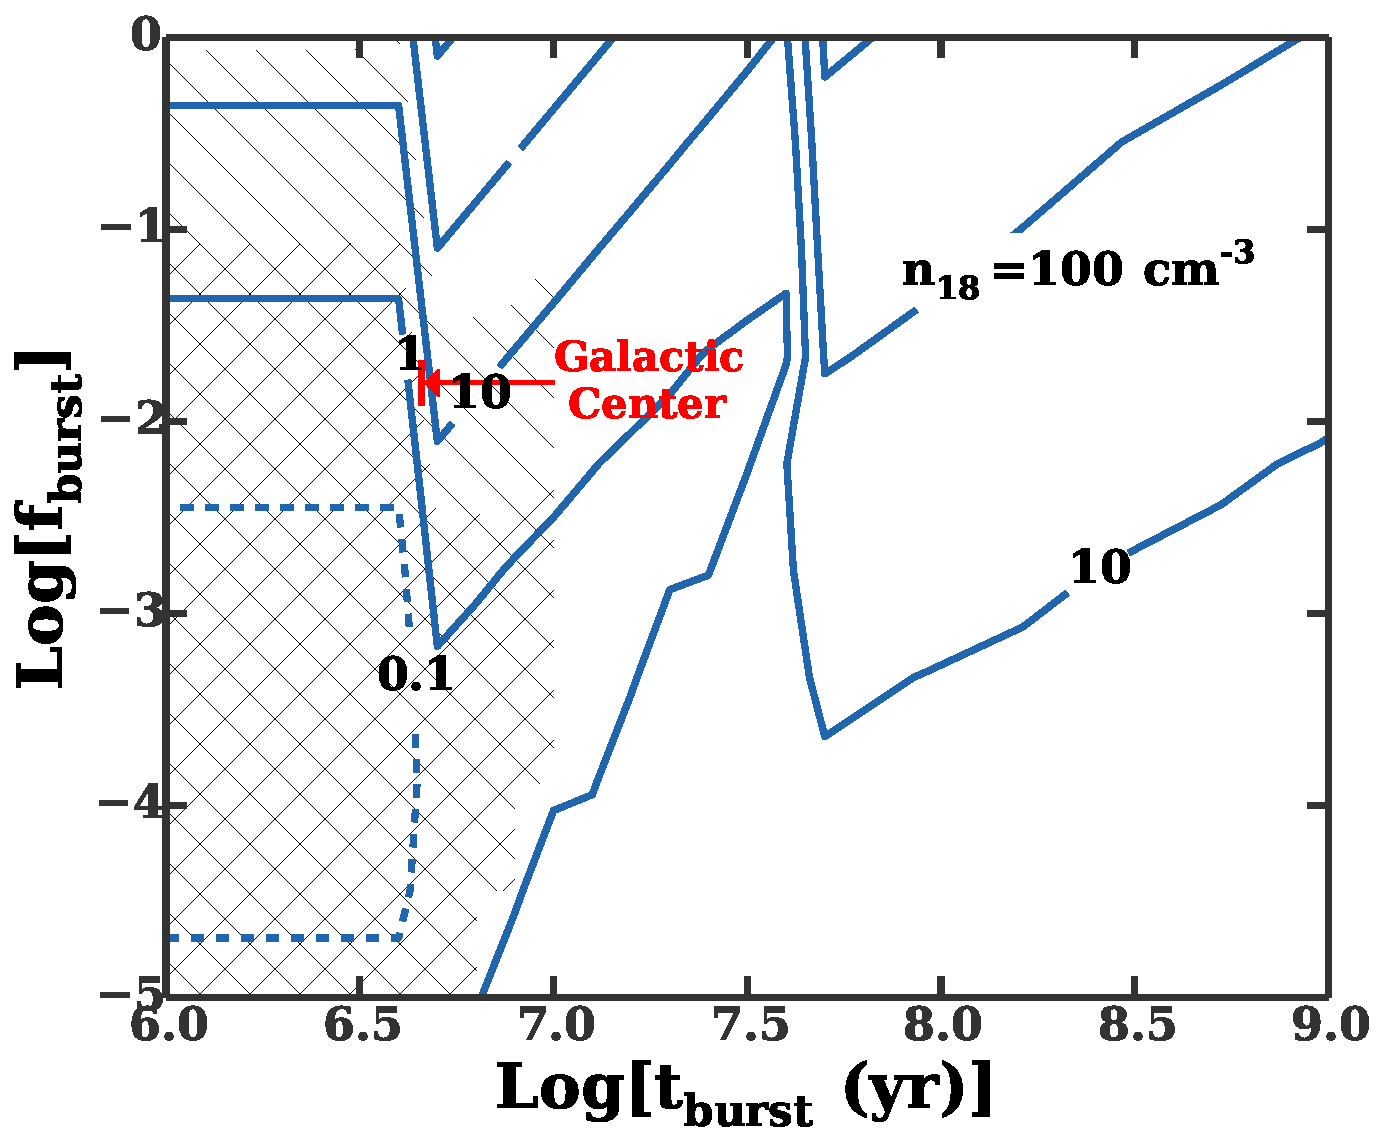
\includegraphics[width=8cm]{cnm_plot.pdf}
  \caption{\label{fig:param} Heating rates ($v_w$) and mass return
    parameters ($\eta$) for different star formation histories (gray
    lines). The solid, gray line corresponds to a star-burst of $<3$ Myr
    ago forming a fraction $f$ of the stars. The rest of the stars
    formed either a Hubble time ago. The fraction $f$ increases and
    the gas density from left to right along these lines. The dashed,
    gray line corresponds to an alternate scenario in which there are
    two recent bursts in rapid succession in rapid succession: the
    older burst is $\sim 3$ Myr old (just at the point when stars are
    beginning to leave the main sequence). The contribution of this
    older burst increases towards the right, approaching the 
    thermally unstable (``TI'') region below the thick black
    line. Iso-contours for the density at $10^{18}$ cm
    ($\mathrm{n_{18}}$) are shown as solid blue lines.}
\end{figure}


\subsection{Empirical Constraints on CNM Density}

In this section we translate observed constraints on the accretion
rate distribution of supermassive BHs into constraints on the CNM
density.  The density $n$ at radius $r$ can be written in terms of the
inflow rate, $\dot{M}$
\begin{equation}
\dot{M} = m \dot{M}_{\rm Edd}= f_{\rm in} 4 \pi r^2 \mu m_p n v,
\label{eq:mdot}
\end{equation}
where $n$ is the average density at radius $r$ and $f_{\rm in}$
represents the fraction of the large scale inflow, which actually
accretes onto the black hole.  If we assume that $r$ is interior to
the sonic radius, then we can approximate $v$ as the free-fall
velocity, $v_{\rm ff} = (2 G \Mbh/r)^{1/2}$.  In this case we
obtain
\begin{equation}
n_{18} = 3 \times 10^3 M_{\bullet,7}^{1/2} m f_{\rm in}^{-1} {\rm
  cm}^{-3}
\label{eq:n18Edd}
\end{equation}
We expect that $f_{\rm in}$ could be quite small for highly sub
Eddington systems. For example, Faraday rotation measurements
\citep{Quataert+2000} show $f_{\rm in}\approx 10^{-3}$, in our own
galactic center. However, we expect $f_{\rm in}$ will be of order
unity for systems with $m\gsim 0.1$.  

\citet{Kauffmann&Heckman2009} present distributions of the OIII line
luminosity, ${\rm L[OIII]}/\Mbh$, for a range of BH masses
($10^7-10^{8.5} \Msun$) from SDSS galaxies.  Assuming a bolometric
correction, these can be translated into distributions of Eddington
ratio $m$.  According to \citet{Kauffmann&Heckman2009} ${\rm
  L[0III]}/\Mbh=1.7$, roughly corresponds to Eddington ratio of 1. We
adopt this conversion and assume that the bolometric correction is
independent of ${\rm L[0III]}/\Mbh$. 

The distribution of Eddington ratios for the lowest mass BH bin of
$M_{\bullet} = 10^7 - 10^{7.25} \Msun$ (\citealt{Kauffmann&Heckman2009};
their Figure 4) is well fit by the expression,
\begin{align}
  F_{\rm cum}(m)=\frac{F_{m_0}}{2^{-1/s}}
  \left[\left(\frac{m}{m_0}\right)^{-a_1\,
      s}+\left(\frac{m}{m_0}\right)^{-a_2 \, s}\right]^{-1/s} \label{eq:khFit},
\end{align}
where $\{s, a_1, a_2, F_{m_0}\} =\{1.42, -0.166, -1.20, 0.235\}$.

\begin{figure}
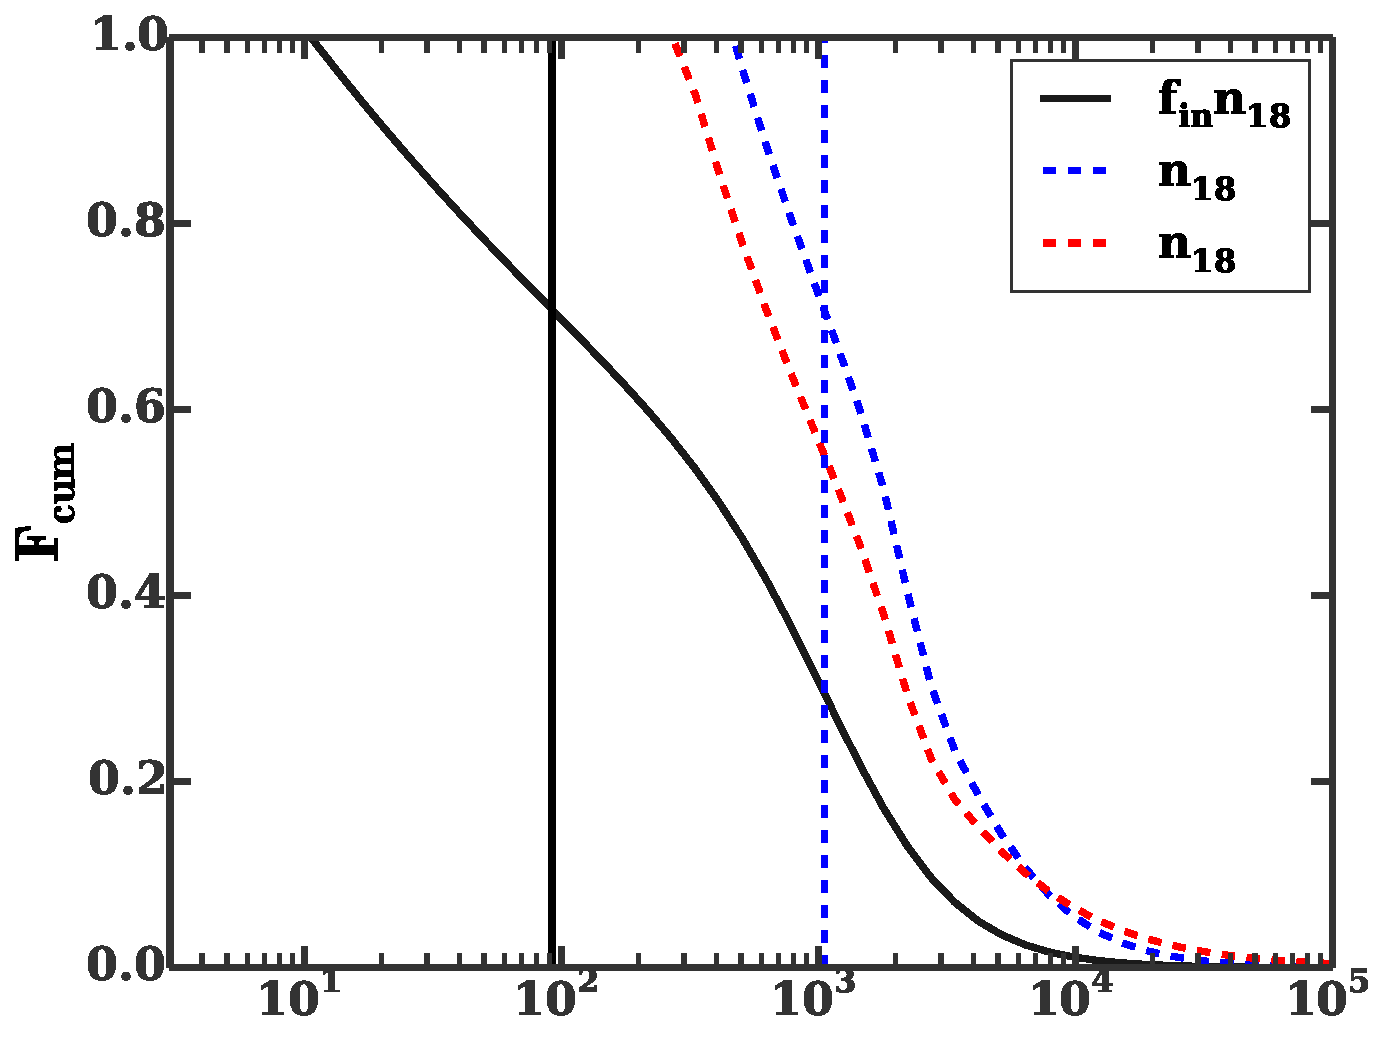
\includegraphics[width=8cm]{fcum_n18.pdf}
\caption{\label{fig:n18Cum} Cumulative distribution of $f_{\rm in}
  n_{18}$ for black holes with mass $\Mbh\simeq 10^{7} \Msun$ based on
  the observed cumulative distributions of Eddington ratios from
  \citet{Kauffmann&Heckman2009} {\it (solid black line)}. Recall that
  $f_{\rm in}$ is the ratio of the true accretion rate onto the black
  hole to the inflow rate of free-falling gas at $10^{18}$ cm.  The
  dashed blue line is the corresponding cumulative distribution of
  $n_{18}$, taking an $f_{\rm in}$ based on the simulations of
  \citet{Li+2013} ($\dot{M}_{\rm Acc}/\dot{M}_{\rm Bondi}$ in their
  Figure 6). The distribution of $f_{\rm in} n_{18}$ ($n_{18}$) is
  unreliable to the left of the solid black (dashed blue) vertical
  line. Such low densities correspond to systems with very small OIII
  luminosities, which could be coming from star formation rather than
  the black hole accretion flow}
\end{figure}


Fig.~\ref{fig:n18Cum} shows the distribution of $n_{18}$ resulting
from combining this distribution with equation~\eqref{eq:n18Edd}.  The
absence of galaxies with $f_{\rm in }n_{18} \lsim$ few cm$^{-3}$
places a lower bound on $n_{18}$ of a few cm$^{-3}$.  However,
measurements of Eddington ratio below $\sim 10^{-3}$ (shown with a
vertical line in Fig.~\ref{fig:n18Cum}) are not reliable. This allows a
moderate fraction of galaxies ($\sim 30\%$) to have much lower gas
densities.


In order to obtain the cumulative distribution for $n_{18}$, we need a
prescription for $f_{\rm in}$. We refer to \citet{Li+2013}, who
performed two-dimensional hydro-dynamical simulations of axi-symmetric
rotating accretion flows. When the inflow rate on large scales was
very sub-Eddington ($\dot{M}/\dot{M}_{\rm Edd} \lsim 10^{-4}$),
cooling was inefficient and $f_{\rm in}$ was $\sim 0.01$. On the other
hand, when $\dot{M}/\dot{M}_{\rm Edd}\gsim 10^{-2}$, $f_{\rm in}$
approaches unity.  We use $\dot{M}_{\rm Acc}/\dot{M}_{\rm Bondi}$ in
their Figure 6 for $f_{\rm in}$.  With this choice only a third of
nuclei have $n_{18}>2,000$ and only 6\% have $n_{18}>10^{4}$. Note
that existing tidal disruption event candidates are unlikely to be in
the high density tail with either no sign or sign of or very weak AGN
emission lines (e.g. \citealt{van-Velzen+2011, Arcavi+2014}). Active
galaxies are generally excluded, so that the TDE sample is not
contaminated by AGN flares.

Note that \citet{Li+2013} use an alpha viscosity prescription with
$\alpha=0.01$.  $f_{\rm in}$ would depend on this choice. This
uncertainty in $f_{\rm in}$ translates into a systematic uncertainty
in the distribution of $n_{18}$. 
 
Two potential complications to keep in mind are (i) clumpiness of the
CNM and (ii) anistropy. The distributions above are distributions of
the {\it average} $n_{18}$.  Most likely, some of the nuclear gas in a
low density hot phase, while the rest is in high density cold
clumps/filaments.  However, while the jet is relativistic the
light-curve of a jet propagating through a clumpy medium will differ
little from that of a smooth medium with the same average
density. Even in the late stages when the jet becomes non-relativistic
clumps will only make a difference when the size of the clumps is
comparable to the size of the jets.

The cold gas could be distributed anistropically. For example it could
be could be concentrated in a ring-like structure. In this scenario,
the some fraction of jets would likely be stifled by the very dense
ring. However, such a ring would not block all jet propagation
directions. 

There may also be anisotropies present in the hot phase of gas. AGN
feedback would may blow low density bubbles in the
CNM. \citet{Russell+2013} used Chandra x-ray observations to measure
gas density and temperature profiles for a sample of massive
elliptical galaxies. The measured electron density on scales of $\sim
100$ pc is $\gsim 0.1$ cm$^{-3}$. Note that the gas density at 100 pc
would be irrelevant for a TDE jet, but we would not expect the gas
density to be decreasing towards the galactic center in a steady
state.  We note that massive black holes in the \citet{Russell+2013}
sample, with $\Mbh\sim 10^{9} \Msun$, whereas black holes tidal
disruption events would have $\Mbh\lsim 10^8 \Msun$. This is because
more massive black holes would not be able to disrupt (main sequence)
stars.


These empirical constraints nicely complement the analytic estimates
in the previous section. On the one hand, the distribution of
Eddington ratios becomes unreliable for low luminosities.  In this
case it is difficult to put a lower bound on the density
observationally. However, the analytics give a low density floor
expected from injection of stellar wind material ($\sim 0.1$
cm$^{-3}$). On the other hand, the analytic estimates are specific to
the hot phase of gas. The Eddington ratio distribution probes the
average density (including any cold clumps). The
distribution of Eddington ratios gives us confidence in our high
density limit ($\sim 1000$ cm$^{-3}$).



\section{TDE jets}
\label{sec:jet}

\subsection{Analytic Considerations}
\label{sec:analytic}


The mass of CNM swept up by the jet $2\pi\theta_{\rm j}^{2}\int m_p
n_{\rm cnm}(r) r^{2}dr$ equals its own rest mass $M_{\rm j} = E_{\rm
  j}/\Gamma_{\rm j}c^{2} \approx \frac{E_{\rm iso}
  (\theta_j^2/2)}{\Gamma_j c^2} $ at the characteristic (`Sedov')
radius given by

\begin{equation}
r_{\rm sedov} = E_{54}^{1/2} \Gamma_{10}^{-1/2} n_{\rm 18}^{-1/2}\,{\rm pc}, 
\end{equation}

where $E_{54}$ is the isotropic equivalent jet energy normalized to
$10^{54}$ ergs. We use our fiducial CNM density profile $n(r)=n_{18}
\left(r/10^{18} {\rm cm}\right)^{-1}$.

From the continuity equation, the (co-moving) density of the jet is
given by (e.g. Uhm \& Beloborodov 2007)
 \begin{align}
   n_{\rm j} =  \frac{L_{\rm j, iso}}{4 \pi r^{2}\Gamma_{\rm
       j}^{2}c^{3}m_p(1 + r \dot{\Gamma_{\rm j}}/c\Gamma_{\rm j}^{3})}
   \approx  \frac{L_{\rm j, iso}}{4 \pi r^{2}\Gamma_{\rm j}^{2}c^{3}m_p}
\end{align}

where the second term in the denominator is generally negligible as
long as the Lorentz factor of the jet changes slowly
$\dot{\Gamma}_{\rm j} \ll c\Gamma_{\rm j}^{3}/r$, as can be shown to
be true at radii $r < r_{\rm sedov}$ as long as $\Gamma_{\rm j}$
changes on timescales $\gtrsim t_{\rm j}$.

A critical parameter is the ratio of the density of the jet to the
CNM

\begin{equation}
  f\approx 40\,  L_{\rm j,48} n_{18}^{-1} \Gamma_{10}^{-2} \, \left(\frac{r}{10^{18} {\rm
        cm}}\right)^{-1} 
\end{equation}

For a given $f$, the Lorentz factor of the shocked material may be
calculated using the relativistic shock jump condition and pressure
equality between the forward and reverse shocks. In the
ultra-relativistic limit

\begin{equation}
\Gamma_{\rm sh} \underset{\Gamma_{\rm sh} \gg 1}= \Gamma_{\rm j}\left[1 + 2\Gamma_{\rm j}f^{-1/2}\right]^{-1/2}
\end{equation}

However, this expression is problematic when the outflow is mildly
relativistic or non-relativistic. In particular, it gives Lorentz
factors less than 1. A more general expression for $\Gamma_{\rm sh}$
can be obtained using equation 3 from \citet{Beloborodov&Uhm2006}

\begin{align}
&\frac{\Gamma_j^2-1}{\gamma_{43}^2-1} f^{-1}=1\\
&\gamma_{43}=\Gamma_j \Gamma_{\rm sh} \left(1-\beta_{\rm sh} \beta_j\right).
\label{eq:gammaShGen}
\end{align}

We use this expression to find the Lorentz factor when the reverse
shock crosses the bulk of the ejecta.  At a given snap-shot in time,
we have the Lorentz factor of the reverse shock (in the lab frame)

\begin{equation}
\Gamma_{\rm rs}=\frac{\beta_{\rm sh}(f)-\beta_{43}(f)/3}{1-\beta_{\rm
    sh}(f) \beta_{43}(f)/3}.
\end{equation} 

Then it is straightforward for a jet of a given thickness, $\delta$,
to find the radius where the reverse shock crosses the trailing edge
of the jet. Then using equation~\eqref{eq:gammaShGen}, we can find the
Lorentz factor of the shocked jet material at the time the reverse
shock has crossed through the jet.  

We plot the fraction of the slow component ($\Gamma_j=2$) kinetic
energy dissipated by the reverse shock as a function of isotropic jet
luminosity and $n_{18}$ in Fig.~\ref{fig:diss}. For the purposes of
our analytic estimates, we assume a constant luminosity jet, which
shuts off after time $t_{\rm fb}=5 \times 10^{5}$ s. For the numerical
calculations described in the subsequent sections, the jet luminosity
declines as $t^{-5/3}$ after time $t_{\rm fb}$ (see equation~\eqref{eq:lum}).


\begin{figure}
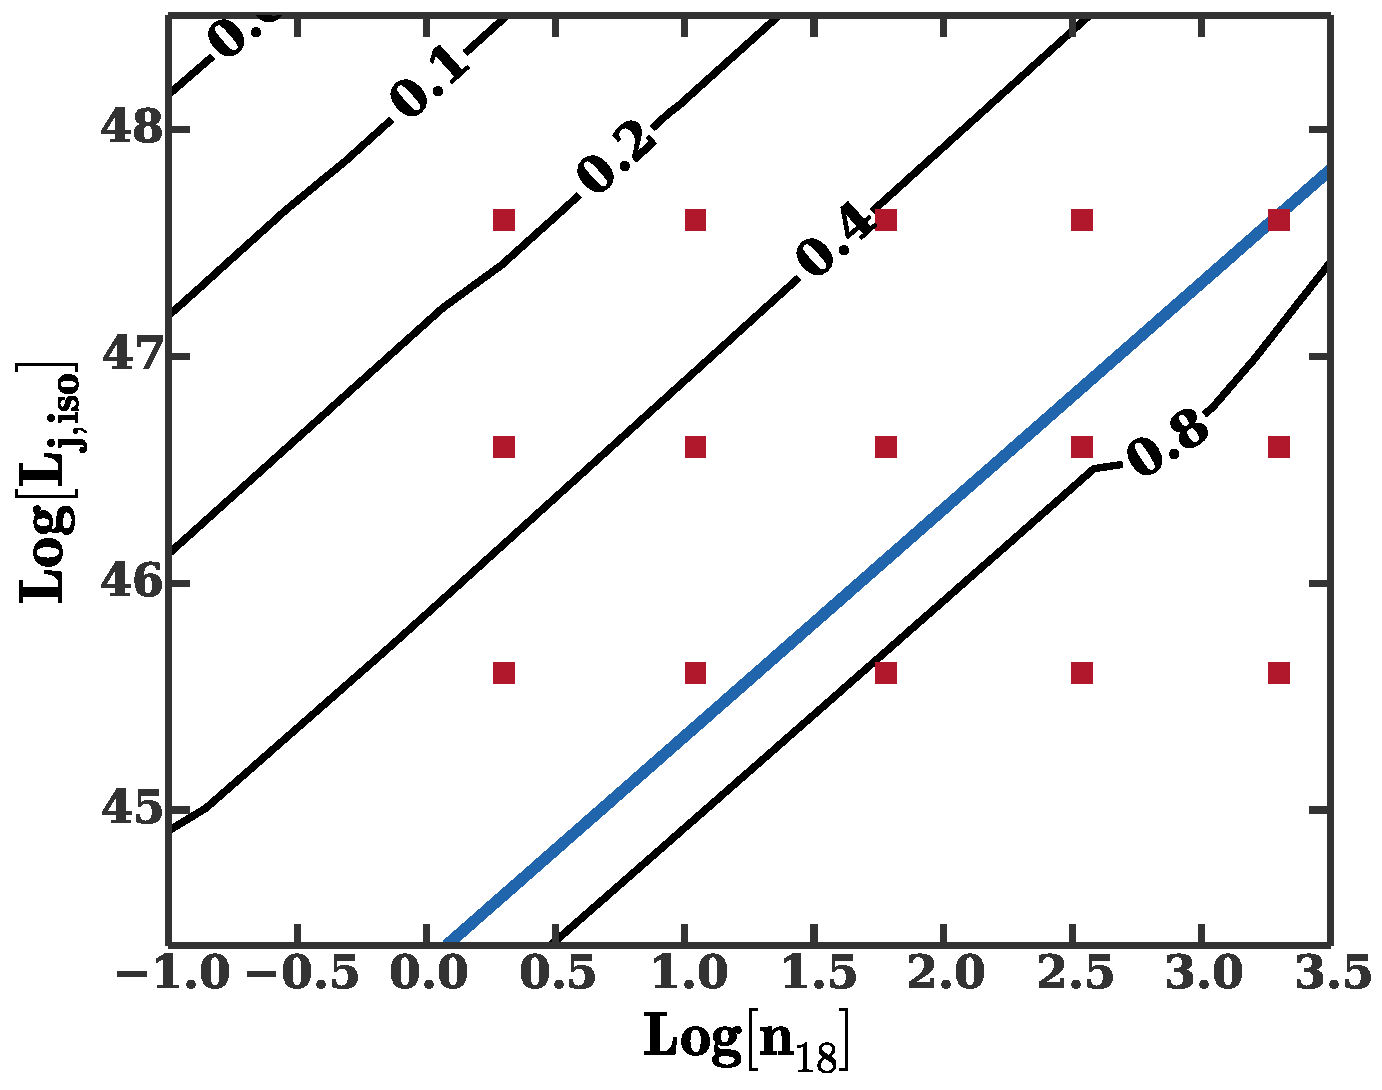
\includegraphics[width=8cm]{diss.pdf}
\caption{\label{fig:diss} Fraction of the slow component
  ($\Gamma_j=2$) kinetic energy dissipated by the reverse shock
  vs. the isotropic jet luminosity ($L_{\rm j,iso}$) and $n_{18}$.}
\end{figure}

\subsection{Jet Models}
\label{sec:numerical}

The jet-CNM interaction is simulated using one and two-dimensions, and
the resulting synchrotron emission is computed using the same
procedure described in \citet{Mimica+2015}. We assume the same angular
Lorentz factor dependence as in previous paper (i.e., $\Gamma = 10$
for the fast inner core and $\Gamma = 2$ for the slow outer sheath),
but we introduce a number of modifications regarding the jet energy
when performing 1D simulations.

\subsection{1D vs. 2D Models}
\label{sec:2d}

The preferred numerical model for Swift J1644+57 \citep[Fig.10
in][]{Mimica+2015} was obtained using 2D simulations (the red line in
that figure). However, the light curve of a 1D version of the same
model \citep[black line in Fig. 10 in][see also section 4.2 of that
paper]{Mimica+2015} matches the 2D light curve only at early times,
when the emission from the inner relativistic jet dominates, while at
late times, when the emission from the slow outer core dominates, the
1D model overestimates the emission from the 2D model. In this work we
found a modification of the 1D model that made its light curves
match the 2D results much more closely.

We first summarize the two-component model as presented in
\citet{Mimica+2015}. We assume that the fast inner core spans an
angular interval $[0, 0.1\ {\rm rad}]$, while the slow outer sheath
occupies $[0.1\ {\rm rad}, 0.5\ {\rm rad}]$. For both components we
assume $E_{\rm ISO} = 4\times 10^{54}$ erg. The crucial thing to
notice is that, keeping $E_{\rm ISO}$ constant, the true jet energy
depends only on the angular interval: $E_{\rm jet} = E_{\rm ISO}
(\cos\theta_{\rm j,min} - \cos\theta_{\rm j,max})$. Note that the
hydrodynamic evolution of the components is independent of angle in 1D
simulations, but the radiative transfer/light-curve calculation is
sensitive to the jet geometry.

Second, we note that, although the sheath is injected in a relatively
narrow angular interval, at late stages of the jet evolution the bow
shock created by its ineraction with CNM spans a much larger interval,
i.e. the slow component becomes almost isotropic \citep[bottom two
panels in Fig. 8 in][]{Mimica+2015}. This is the reason for the
discrepancy with the 1D simulation, because there the slow component
angular size is fixed to the initial one. We note that the stage at
which the jet becomes ``isotropic'' depends on the CNM density,
i.e. the denser the CNM, the faster this is expected to happen.

Since the agreement between 1D and 2D models is good at the early
times (when the fast component dominates), we modify only the slow
component in 1D models. We assume that is spans $[0.1\ {\rm rad},
\pi/2\ {\rm rad}]$ and lower its $E_{\rm ISO}$ so that the true jet
energy remains unchanged with respect to the original model:
\begin{equation}\label{eq:Eiso}
 E_{\rm ISO, new} = E_{\rm ISO} \left(\frac{\cos(0.1) - \cos(0.5)}{\cos(0.1) - \cos(\pi/2)}\right)\approx 0.12 E_{\rm ISO}\, .
\end{equation}

We assume $E_{\rm ISO} = 4\times 10^{54}$ erg, and that the jet
luminosity time dependence is the same as in \citet{Mimica+2015},
\begin{equation}\label{eq:lum}
L_j(t) = L_{j,0}\max\left[1, (t/t_0)\right]^{-5/3}
\end{equation}
where $t_0 = 5\times 10^5$ seconds and $L_{j, 0}$ can be determined
from $E_{\rm ISO}$ by integrating equation~\ref{eq:lum} in time from
$0$ to $\infty$. We show a comparison of this modified 1D approach
with the true 2-d result in Figure~\ref{fig:1d2dB}, for $n_{18}=60$
and $n_{18}=2000$. For $n_{18}=2000$ the agreement is excellent, while
for $n_{18}=60$ the 1d models still over-predict still over-predict
the flux at times after the peak of the light-curve.


\begin{figure*}
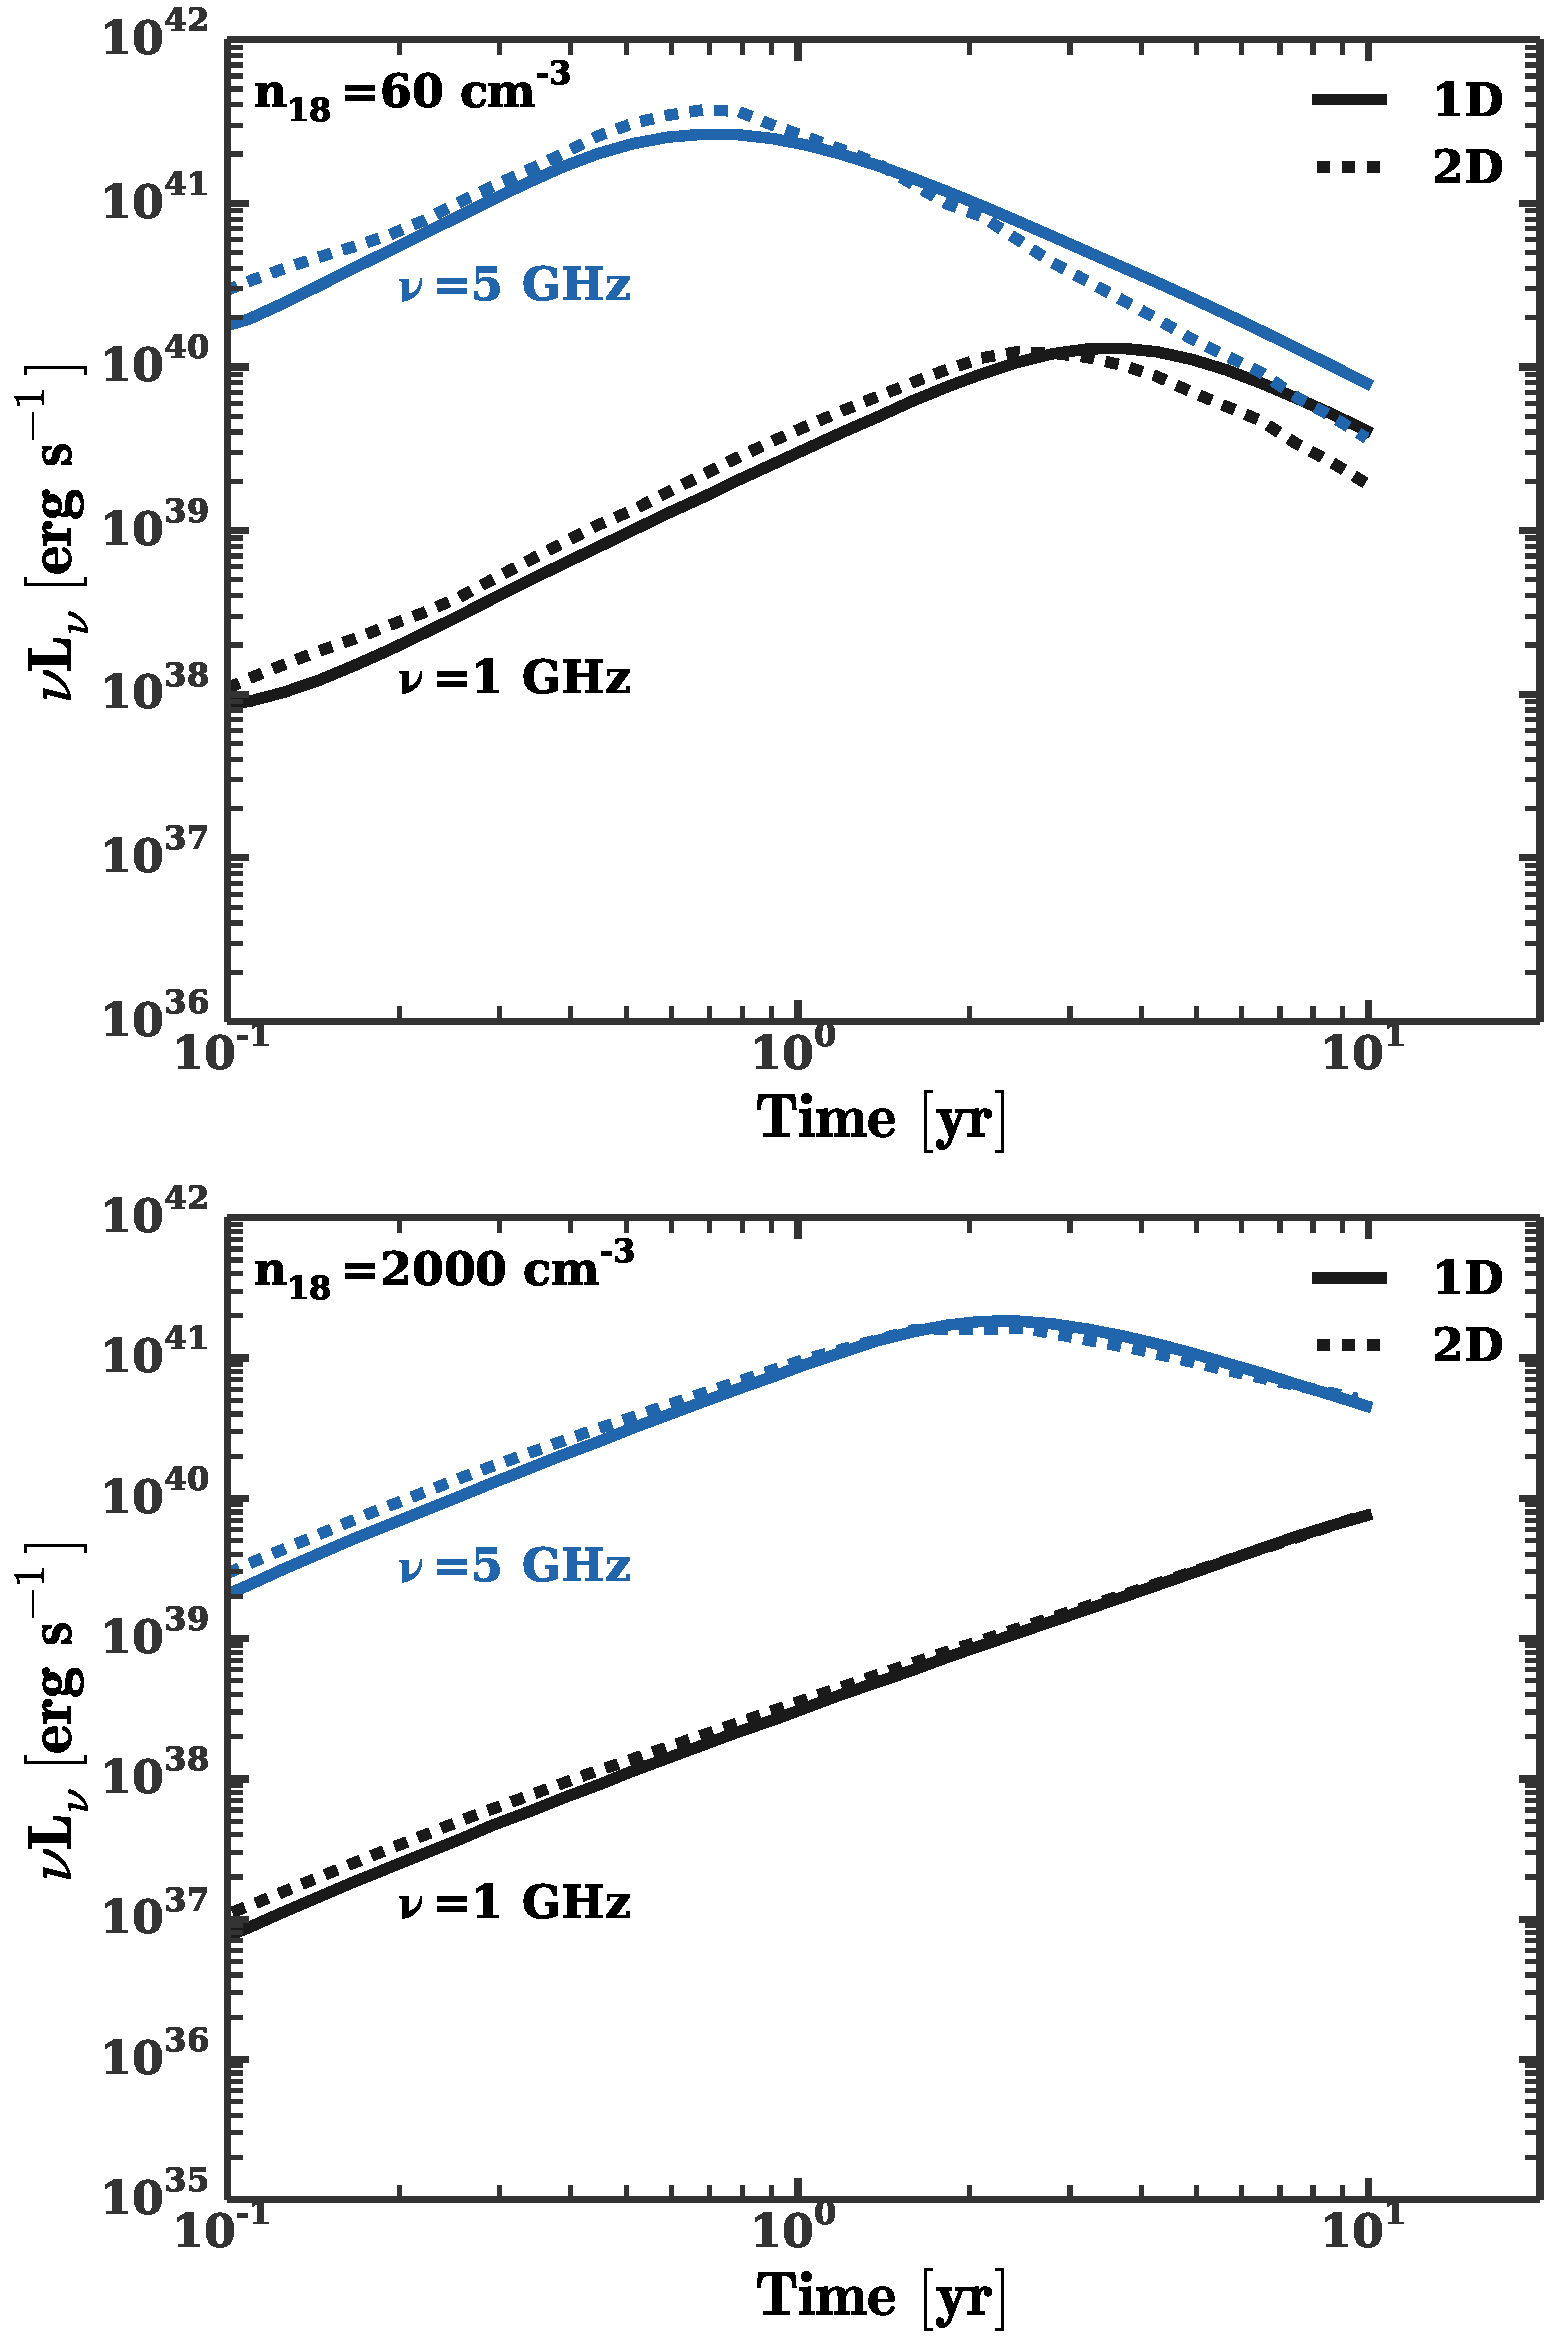
\includegraphics[width=16cm]{1d_2d.pdf}
\caption{\label{fig:1d2dB} Comparison of 1D and 2-d light-curves for
  $n_{18}=60$ (top) and $n_{18}=2000$ (bottom) for frequencies of 1
  GHz (left) and 30 GHz (right) and an observer angle of 0.8 radians
  to the jet axis. We assume an $n\sim r^{-1}$ density profile for
  $n_{18}=2000$, but take $n\sim r^{-1.5}$ for $n_{18}=60$ for
  computational convenience--this model was previously computed in
  \citet{Mimica+2015} and 1D results suggest that the density slope would
  have minimal impact on the results (see $\S$~\ref{sec:profileComp})}.
\end{figure*}

\section{Results}
\label{sec:results}

\subsection{Effect of gas density}

In Fig.~\ref{fig:upper_limits} we show off-axis light curves for our
fiducial jet model and a few different densities: n$_{18}$: 2,
60, and 2000 cm$^{-3}$. The higher density models peak at later times with
smaller peak luminosities.  This is due to the effects of synchrotron
self-absorption: the peak of the emission occurs as the jet
transitions from being optically thick to optically thin. This occurs
later in the higher density models.

The radio light curve has contributions from both the slow and fast
jet components. The fast component dominates at early times for the
$n_{18}=2$ and 60 lightcurves, while the slow component dominates for
all times for $n_{18}$=2000. Generally, the fast
component is more important at higher frequencies, and lower
densities. 

We also show radio upper limits and detections for various TDE
candidates in Fig.~\ref{fig:upper_limits} (these were compiled from
various sources into Table 1 of \citealt{Mimica+2015}). Note that all
of 5 GHz light-curves fall above the upper limits. However, we were
unable to perform a 2-d calculation for $n_{18}=2$.  For $n_{18}=60$,
the 2-d light-curve falls $\sim$one order of magnitude below the 1D
light-curve after $\sim$ 10 years. Thus, we caution that the 1D
light-curves for $n_{18}=2$ may overestimate the late time radio
luminosity.

Overall, earlier radio measurements would provide tighter constraints
for tidal disruption event jets: the lightcurves or $n_{18}=2$ peak on
time-scales of months, while many of the radio measurements were taken
decades after the TDE flare.

\begin{figure} 
  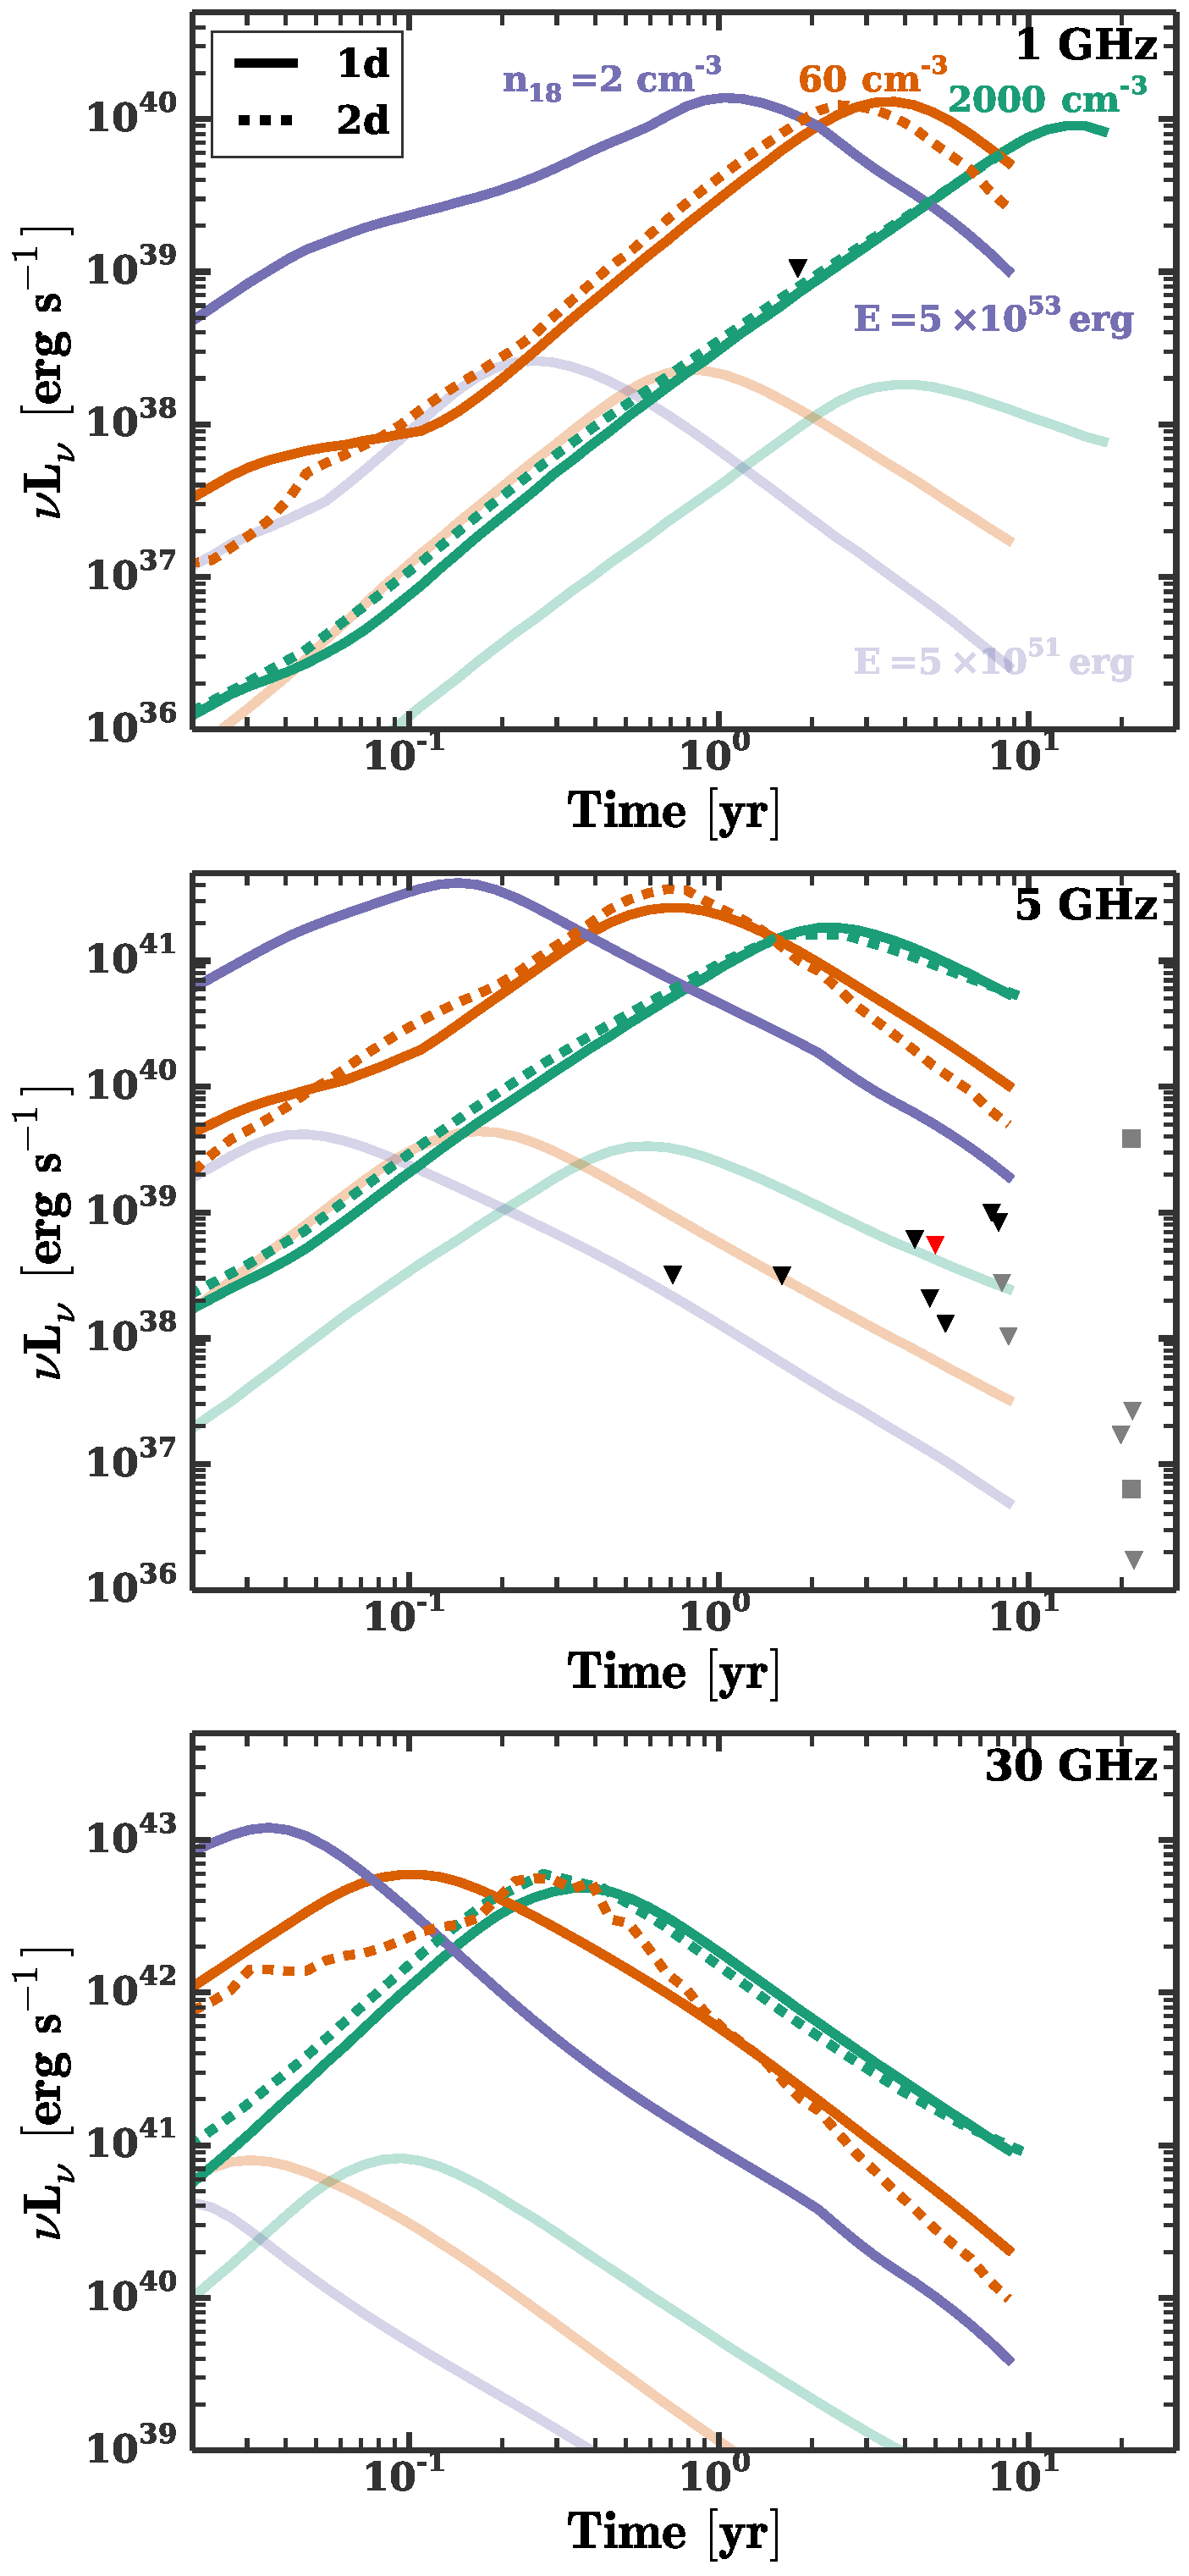
\includegraphics[width=8cm]{lightcurves.pdf}
  \caption{\label{fig:upper_limits} Off-axis ($\theta_{\rm obs}=0.8$)
    radio light-curves for our fiducial jet model and three different
    values of n$_{18}$: 2, 60, and 2000. Solid lines correspond to the
    light-curves from 1D jet simulations. When available ($n_{18}=60$
    and $n_{18}$=2000), we have plotted light curves from the 2D jet
    simulations as dashed lines. Note we use $n\propto r^{-1}$ for
    $n_{18}=$ 2 and 2000, but $r^{-1.5}$ for $n_{18}=60$, as this
    model had already been computed and since the 1D results suggest
    that the density slope will have minimal impact on the results
    (see $\S$~\ref{sec:profileComp}).  Radio upper limits and
    detections are shown as black/gray triangles and squares
    respectively (compiled in Table 1 of \citealt{Mimica+2015}). The
    single upper limit in the top panel corresponds to 1.4 GHz. Gray
    triangles and squares in the middle panel indicate upper limits
    and detections at 3.0 GHz, while black triangles indicate upper
    limits at 5.0 GHz.}
\end{figure}

\subsection{Effect of gas density profile}
\label{sec:profileComp}
We have also computed the radio light-curves for different shapes of
the gas density profile, while holding $n_{18}$ fixed. We compute the
results for $n_{18}=2000$ for both our fiducial $n\sim r^{-1}$ profile and
the core galaxy profile, shown in equation~\eqref{eq:cores}. The
former would more relevant for a cuspy stellar density profile with
stellar density $\rho_{\star}\propto r^{-2}$, while the latter would be more
appropriate for a flatter $\rho_{\star}\propto r^{-1}$ stellar density
profile. As a steeper stellar density is more favorable for producing
tidal disruption events, we would expect most events to occur is cusp
rather than core galaxies.

The on-axis light-curves are virtually indistinguishable as shown in
Fig.~\ref{fig:cores}. This result is not surprising as
the core and cusp profiles are quite similar inside of $10^{18}$ cm,
and we expect the jet to have decelerated inside of this radius for
these high densities. 

In Fig.~\ref{fig:profs2} we compare the 1D on-axis light-curves for
density two density profiles: $n\propto r^{-1}$ and $n\propto r^{-1.5}$
with $n_{18}=60$. Once again the results are quite similar. Again this
is not surprising as the models have the same density near the Sedov
radius ($\sim 10^{18}$ cm).  


\begin{figure} 
  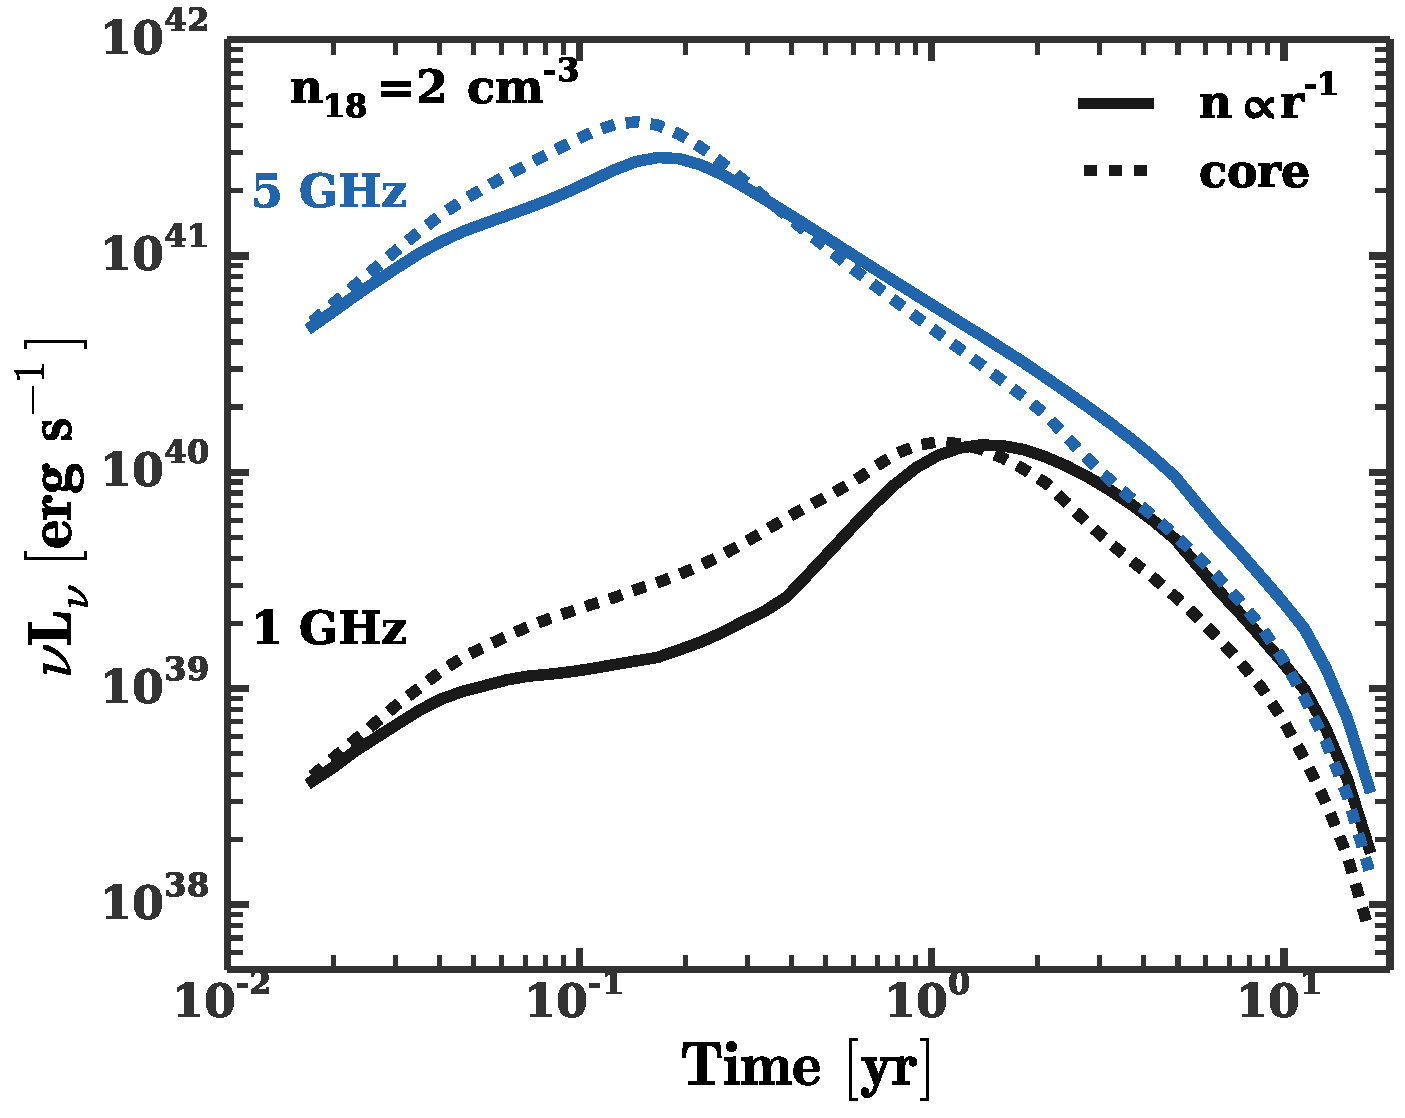
\includegraphics[width=8cm]{fig_cores.pdf}
  \caption{\label{fig:cores} Comparison of (on-axis) light-curves for
    $n_{18}=2000$ and two different CNM gas density profiles: $n\sim
    r^{-1}$ and the core galaxy profile from \eqref{eq:cores} with
    $r_s=10^{18}$ cm and $n(r_s)=2000$, so that we can isolate the
    effect of the shape of the density profile.}
\end{figure}


\begin{figure} 
  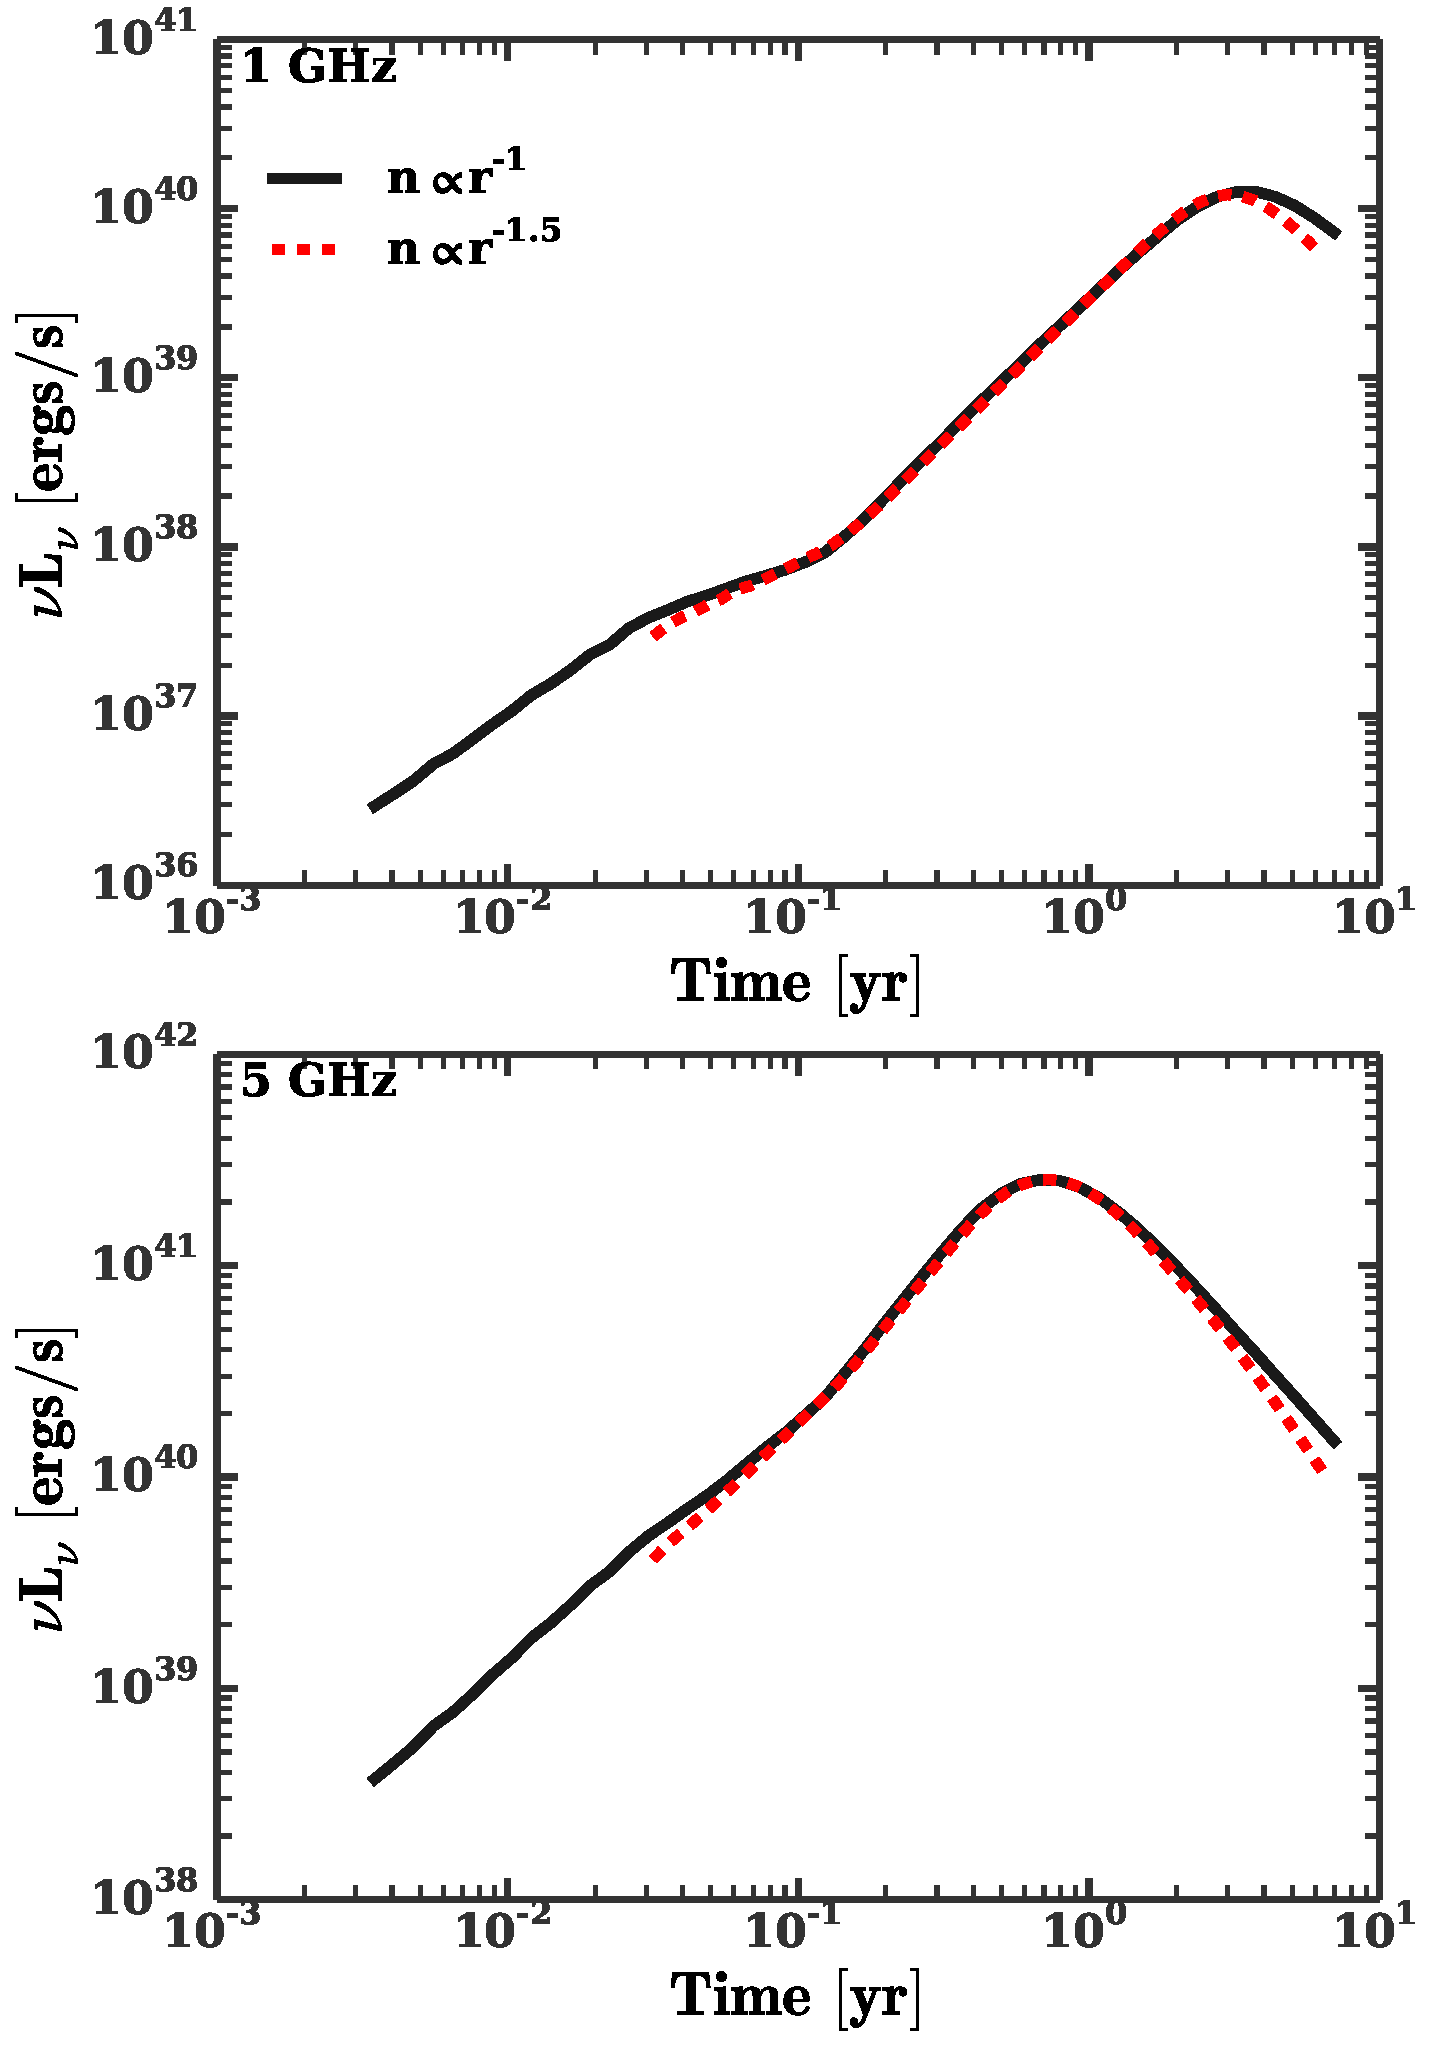
\includegraphics[width=8cm]{profs2.pdf}
  \caption{\label{fig:profs2} Comparison of (on-axis) light-curves for
    $n_{18}=60$ and two different CNM gas density profiles: $n\propto
    r^{-1}$ ({\it solid black}) and $n\propto r^{-1.5}$ ({\it dashed
      red}).}
\end{figure}

\subsection{Effects of viewing angle}
We show a comparison off and on-axis light-curves in
Fig.~\ref{fig:onOff}.  For $n_{18}=2000$ the light-curves differ
little.  For $n_{18}=60$ off-axis luminosity is lower by a factor
before and near the peak. However, for late times
the off- and on-axis light-curves are quite similar.

\begin{figure*}
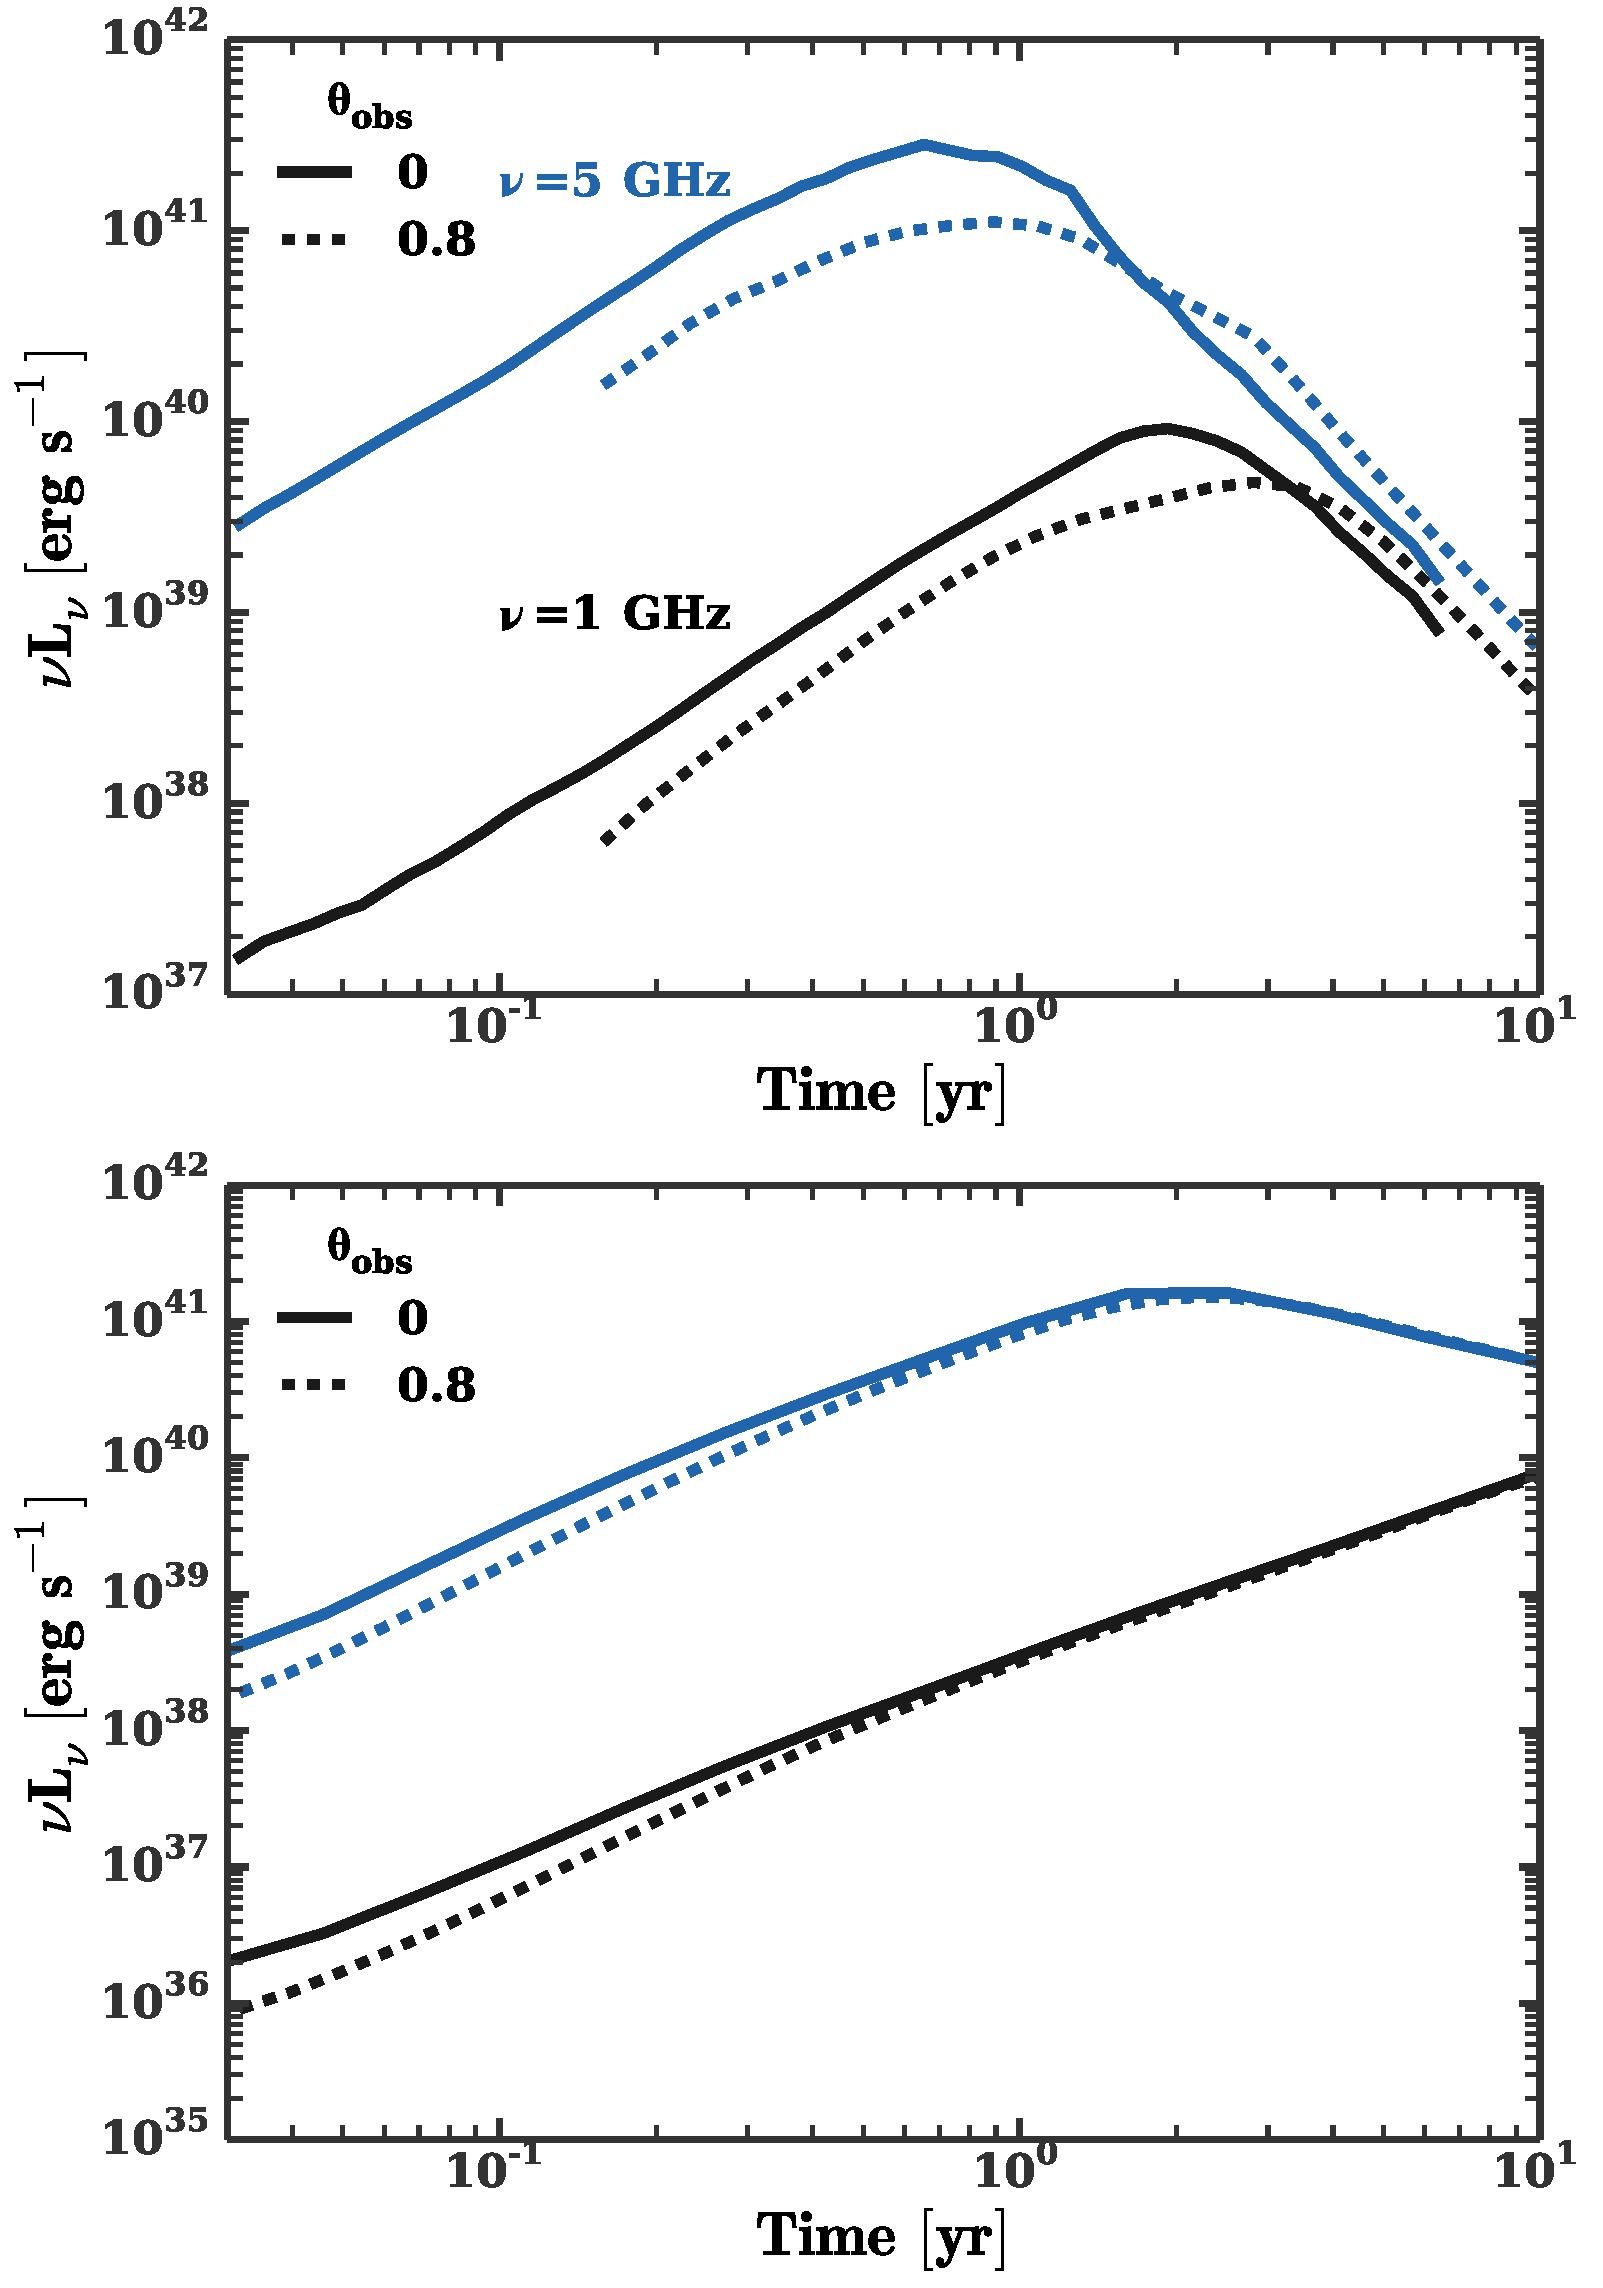
\includegraphics[width=16cm]{on_off.pdf}
\caption{\label{fig:onOff} Comparison of (2D) off- and on-axis
  light-curves for $n_{18}=60$ (top) and $n_{18}=2000$ (bottom) for
  frequencies of 1 GHz (left) and 5 GHz (right). The observer line of
  sight is taken to be at $\theta_{\rm obs}=0.8$ with respect to the
  jet axis. We assume an $n\sim r^{-1}$ density profile for
  $n_{18}=2000$, but take $n\sim r^{-1.5}$ for $n_{18}=60$ for
  computational convenience.}
\end{figure*}



\section{Summary and Conclusions}
\label{sec:conc}

We calculate radio light-curves for tidal disruption event jets
propagating through different circumnuclear (CNM) gas densities. We
simulate the jet propagation using both 1d and 2d hydrodynamic
simulations. We then post-process these to produce radio synchrotron
light-curves. To isolate the effects of the density profile we take a
fixed two component jet model from \citet{Mimica+2015}, which produces
a good fit to the observed radio data in the Sw1644 transient. We
consider a broad range of gas densities motivated by analytic
estimates of stellar wind mass injection and empirical constraints
based on observed distributions of Eddington ratios. Our conclusions
are summarized as follows.

\begin{enumerate}
\item We estimate the hot phase densities expected from injection of
  stellar wind material for different star formation histories. We
  find that that range of gas densities at 10$^{18}$ cm is $n_{18}
  \sim$ 1-1000 cm$^{-3}$.

\item The slope of the gas density profile depends on the slope of the
  stellar density profile. We expect a typical TDE host to have cusp
  like stellar density profile inside of a few pc, with $\rho_\star
  \propto r^{-2}$. This translates into a gas density profile $n
  \propto r^{-1}$. The radio light-curve of a TDE jet is most
  sensitive to the density at the deceleration/Sedov radius (where it
  has swept up its mass in CNM gas). The light-curve will be
  insensitive to changes in slope for fixed density at the
  deceleration radius.

\item We use the distribution of Eddington ratios (measured by
  \citealt{Kauffmann&Heckman2009} using $L[0III]/\Mbh$) for a sample $\sim
  10^{7} \Msun$ black holes from SDSS to obtain an empirical
  constraint on the average circumnuclear gas density, including all
  phases of gas. We find that $\sim90\%$ of galaxies in the sample
  have $n_{18}<10^{4} {\rm cm}^{-3}$, although we note that there is
  considerable uncertainty in translating an observed Eddington ratio
  to a circumnuclear gas density. TDE hosts would not fall on this
  high density tail, as TDE searches exclude galaxies with evidence of
  AGN activity. 

\item We take a jet model which fits the radio data for the Sw1644
  transient (from \citealt{Mimica+2015}) and run it through a range of
  different density profiles. Motivated by the above results for the
  expected range of gas densities we take the density at $10^{18}$ cm,
  to be $n_{18}=2, 60,$ or 2000 cm$^{-3}$. We find bright radio
  emission at a few GHz across this entire range of densities, with
  the peak luminosity only weakly dependent on the chosen value of
  $n_{18}$.  For smaller densities the light-curves peak earlier in
  time. Based on existing radio upper limits for tidal disruption
  event candidates, we show Swift 1644-like jet are absent in most TDEs
  as long as the density at $10^{18}$, $n_{18} \gsim  60$
  cm$^{-3}$. Prompt follow-up in the radio could provide tighter
  constraints on the existence of TDE jets.  
\end{enumerate}

\appendix
\section{Core Profile}
\label{app:core}
In $\S\ref{sec:profileComp}$ we compare the results of radio
light-curves from jets propagating in core and cusp like gas density
profiles. See Fig.~\ref{fig:profiles} for a comparison of core and
cusp-like profiles. 

We use the following analytic expression to approximate the core
galaxy profile

\begin{align}
\begin{cases}
n=n(r_s) k(x) & 0.4 \leq x\leq 2.0\\
n = 2.0 n(r_s) (x/0.4)^{-0.95} & x < 0.4\\
n = 0.75 n(r_s) (x/2.0)^{-0.26} & x>2.\\
\end{cases}
\label{eq:cores}
\end{align}

Where, 

\begin{align}
  &x=r/r_s\\\nonumber
  &k(x)=\frac{45}{19} \frac{1}{x^{3/2}} \frac{1-x^{1.9}}{9-19
      x\frac{x^{0.9}-1}{x^{1.9}-1}}
\end{align}

To isolate the effects of the shape of the density profile, consider a
core density profile with $r_s=10^{18}$ cm, and $n_{18}=2000$: the
same as our high density cusp model.

\clearpage
  \footnotesize{
    \bibliographystyle{mnras}
    \bibliography{master}
  }

\end{document}
